\documentclass[preprint,12pt]{elsarticle}
\usepackage{lmodern}
\ifdefined\pdfgentounicode
\input{glyphtounicode}
\pdfgentounicode=1
\fi
\usepackage{amsmath,amssymb,amsfonts,mathtools,amsthm,bm}
\usepackage{booktabs,graphicx,array,tabularx,longtable,float,url}
\usepackage{needspace}
\usepackage{placeins}
\usepackage[hidelinks]{hyperref}
\hypersetup{pdfauthor={Ali Eslami and Jiangbo Yu}}
\usepackage[protrusion=true,expansion=false]{microtype}
\graphicspath{{figures/}{./}}
\allowdisplaybreaks
\setlength{\emergencystretch}{3em}
\interdisplaylinepenalty=2500
\theoremstyle{definition}
\newtheorem{assumption}{Assumption}
\theoremstyle{plain}
\newtheorem{theorem}{Theorem}
\newtheorem{proposition}{Proposition}
\newtheorem{lemma}{Lemma}
\newtheorem{corollary}{Corollary}
\newtheorem{remark}{Remark}
\theoremstyle{definition}
\newtheorem{definition}{Definition}
\newtheorem{problem}{Problem}
\theoremstyle{plain}
\floatstyle{ruled}
\newfloat{algorithm}{tbp}{loa}
\floatname{algorithm}{Algorithm}
\newcommand{\R}{\mathbb{R}}
% elsarticle includes the word ``Appendix'' in appendix-section references.
\newcommand{\appref}[1]{\ref{#1}}
\newcommand{\longpaperdetails}[1]{#1 of the \href{https://github.com/AlienEslami/agentic-perimeter-runtime-certification/blob/main/paper/main.pdf}{long version}}
\newcommand{\reproductiondetails}[1]{\href{https://github.com/AlienEslami/agentic-perimeter-runtime-certification/releases/tag/paper-2026-11-10}{#1}~\cite{perimeterReproductionGuide}}
\journal{Transportation Research Part B: Methodological}



% Reduced manuscript: certification structure and supporting appendices, 10 November 2026.
\begin{document}
\begin{frontmatter}
\title{Formal Guarantees for Trustworthy Agent-Mediated Urban Perimeter Control}
\author[mcgill]{Ali Eslami}
\ead{ali.eslami@mcgill.ca}
\author[mcgill]{Jiangbo Yu\corref{cor1}}
\ead{jiangbo.yu@mcgill.ca}
\cortext[cor1]{Corresponding author.}
\affiliation[mcgill]{organization={Department of Civil Engineering, McGill University},
 addressline={817 Sherbrooke Street West}, city={Montreal}, state={Quebec},
 postcode={H3A 0G4}, country={Canada}}
\begin{abstract}\fontsize{11}{13}\selectfont
Perimeter control helps reduce urban congestion by regulating traffic flows
between regions. Control plans may need to be revised as traffic conditions
and operating priorities change. Artificial intelligence (AI) agents can
support this process by interpreting operator instructions and using tools
to develop control plans. However, each new agent-proposed plan must remain
compatible with the evolving traffic state, uncertainty, and outstanding
service requirements. In this paper, we develop a dual-agent framework in
which an AI agent proposes plans and a rule-based supervisory agent checks
them before execution. The supervisor verifies whether a proposed plan
respects vehicle conservation, nonnegative traffic states, boundary-storage
limits, and service deadlines under bounded state-estimation and
arrival-forecast errors. It determines whether the plan can be executed as
proposed, needs modification to meet these requirements, or should be
rejected while the current plan continues under its existing guarantee.
We also establish conditions for maintaining these guarantees beyond a
plan's specified duration. Numerical studies show that the framework can
accept plans unchanged, certify more plans by using traffic-specific
structure, and repair proposals to meet the requirements. Further
experiments show that the framework
can accept beneficial changes while rejecting requests that would violate
boundary-storage or service requirements, including under computation
delays and agent-context errors. Overall, the framework supports
trustworthy AI for transportation by connecting adaptive agent decisions
to traffic control that satisfies physical limits and service requirements.
\end{abstract}
\begin{keyword}
Urban perimeter control \sep Macroscopic fundamental diagram \sep Agentic AI \sep Formal guarantees
\end{keyword}
\end{frontmatter}


\section{Introduction}
\label{sec:new-introduction}

Urban perimeter control manages congestion by regulating traffic flows
between regions. Restricting entry to a congested region can
improve traffic conditions inside it, but may also cause queues to grow at
its boundary. Control decisions must therefore account for both regional
congestion and the storage capacity of boundary queues
\cite{haddad2017queues}. One approach to modeling regional traffic uses
the macroscopic fundamental diagram (MFD), which relates the number of
vehicles in a region to its aggregate outflow
\cite{geroliminis2008existence,daganzo2008analytical,geroliminis2011properties}.

Within this modeling framework, feedback control methods adjust boundary
flows in response to observed traffic conditions
\cite{keyvan2012gating,aboudolas2013perimeter}. Predictive methods use the
traffic model and demand forecasts to select control actions over a
planning horizon \cite{geroliminis2013mpc,sirmatel2018economic}. Related
formulations explicitly account for boundary queues and their storage
limits \cite{haddad2017queues}. Robust control methods address uncertain
demand and limited traffic measurements, with stability and robustness
guarantees established under specified modeling assumptions
\cite{zhong2018robust,mohajerpoor2020hinf}. Earlier robust perimeter-control
formulations also address MFD uncertainty and uncertain destination
decomposition, including constrained interpolation-based control
\cite{haddad2014robust,haddad2015robust}.

Data-driven approaches have also been developed for perimeter control.
Reinforcement learning and adaptive dynamic programming use traffic
observations and the outcomes of control actions to learn control policies
\cite{chen2022dataefficient,chen2024iadp}. Multi-agent reinforcement
learning supports coordination across several regions and allows
different metering rates at individual boundary signals
\cite{zhou2023scalable,yu2025physicsperimeter}. Other formulations consider
controllers with different objectives. For example, Li et al.\ \cite{li2024beyond}
study non-cooperative interactions between controllers managing perimeter
flows and traffic generated within the network.

AI agents can also support traffic management by interpreting operator
instructions and using tools to develop control plans. TrafficGPT and
Open-TI demonstrate natural-language interaction with specialized
traffic-analysis tools \cite{trafficgpt2024,openti2024}. LA-Light couples
a large language model (LLM) with traffic-signal tools and checks the format of its proposed
decisions \cite{wang2024lalight}. Similar arrangements have been explored in robotics: SayCan connects language
instructions to robot skills \cite{saycan2023}, while VoxPoser uses
language-derived objectives and constraints to guide motion planning
\cite{voxposer2023}. For perimeter control, these precedents motivate
investigating agents that interpret instructions about regional priorities
and their duration, and use tools to develop and revise control plans.

An agent may use a planning tool with the wrong objective or base its
request on incorrect context. Even when the objective is appropriate, a
plan that satisfies the constraints in simulated cases may violate them
for other allowed initial states or arrival patterns. Traffic also
continues to evolve while a plan is being computed and checked, so a
replacement must be assessed for the conditions at the time of
implementation. These concerns distinguish the agent's interpretation of
an instruction from the checks needed before a plan can be executed.

Existing assurance methods provide several relevant foundations
\cite{hobbs2023runtime}. Simplex architectures retain a verified backup
when a proposed control action cannot be accepted \cite{mehmood2022black}.
Control barrier functions enforce prescribed state constraints
\cite{ames2017}, while predictive safety filters assess future behavior
and modify proposals to preserve feasibility \cite{wabersich2021}.
Shielding uses a model and a formal specification to restrict a learner's
actions \cite{alshiekh2018}. Formal traffic-control methods exploit mixed
monotonicity to over-approximate reachable states and synthesize controllers
satisfying temporal-logic specifications \cite{coogan2017formal}.
Related reachability methods retain dependencies between uncertain states
\cite{coogan2020mixed,kochdumper2021sparse}. For LLM agents, specifications
on data flows and tool sequences provide a further level of runtime
enforcement \cite{doshi2026tools}.

The perimeter-control studies reviewed above do not provide a framework
that checks agent-proposed plans against both boundary-storage limits and
fixed service deadlines under uncertainty, while preserving these
guarantees when plans are replaced, rejected, or delayed. Addressing this
gap requires checks that account for the nonlinear traffic dynamics and
the states that can arise before a replacement starts.

We consider two urban regions described by an MFD-based traffic model,
with an exterior queue for vehicles waiting to enter the network. An AI
agent uses planning tools to propose control plans, and a rule-based
supervisory agent checks them before execution. Together, they form the
dual-agent architecture studied here. The supervisor determines whether
each proposed plan can replace the current plan while respecting physical
limits and meeting pending service deadlines. Traffic information,
physical limits, and service requirements are supplied to the tools and
supervisor independently of the AI agent's requests.

We develop guarantees under the stated traffic model, allowing for
state-estimation errors at the time a plan starts and errors in arrival
forecasts. The supervisor bounds future regional vehicle counts and
boundary queues, then checks physical constraints throughout the plan and
service requirements at their deadlines. These checks apply to new plans
proposed while the current plan is being executed and account for traffic
evolution during computation. When a replacement is rejected or late,
the current plan continues for the period covered by its certificate.

The paper makes three main contributions:
\begin{enumerate}
\item We develop a method to bound regional vehicle counts and boundary
queues under uncertainty. By using vehicle conservation and the
relationships between uncertain traffic quantities, the method gives
tighter bounds for checking physical limits and service deadlines. It
also applies to networks with several entry queues.

\item We establish physical and service guarantees as plans are replaced,
including delays in computation and continued use of the current plan
after rejection. These guarantees hold for arbitrary agent requests under
the stated traffic and interface assumptions. We also give conditions
under which they can continue beyond the planned control period.

\item We develop a repair procedure that tests plans between a proposal
and a certified backup. It identifies the certified candidate with the
smallest control-input change among the tested alternatives, while the
current plan remains in use if no replacement is ready in time.
\end{enumerate}

Section~\ref{sec:new-problem} presents the traffic model and control
problem. Section~\ref{sec:new-agent} describes the two agents and their
planning and execution interface. Section~\ref{sec:new-certification} develops the
certification procedure and execution guarantees, with their proofs.
Supporting terminal-continuation and repair-cost proofs are included in
the appendices.
Section~\ref{sec:new-evidence} presents the numerical studies,
Section~\ref{sec:new-discussion} discusses operational implications, and
Section~\ref{sec:new-conclusion} concludes the paper.

\section{Two-Region MFD Perimeter-Control Problem}
\label{sec:new-problem}

\subsection{Traffic dynamics}
\label{app:new-model}

We consider two urban regions and an exterior entry queue, as shown in
Figure~\ref{fig:two-region-network}. Region~1 exchanges traffic only
with Region~2, which also borders the exterior. The accumulation $n_{ij}(t)$ counts
vehicles currently in region $i\in\{1,2\}$ with destination
$j\in\{0,1,2\}$, where $0$ denotes the exterior. The regional total is
$n_i=\sum_{j=0}^2n_{ij}$, and $z(t)$ is the queue waiting to enter
Region~2. Accumulations are measured in vehicles, time in hours, and all
flow rates in veh/h. The known internal demand $d_{ij}^{\rm int}\ge0$ is the
rate of trips generated inside region $i$ with destination $j$. These
demands remain constant in the studies below.

Each perimeter control input $u_{ij}(t)\in[0,1]$ regulates flow across
the boundary from $i$ to $j$. Its indices identify the boundary, whereas
those of $n_{ij}$ identify current region and final destination. Thus
$u_{12}$ controls both $n_{12}$ and $n_{10}$ vehicles leaving Region~1
for Region~2. Let $G_i(n_i)$ be the regional MFD outflow, and let $a$ be
the admission rate from the queue, with fractions $\pi$ and $1-\pi$
destined for Regions~1 and~2. Exterior arrivals join the queue at rate
$\Lambda(t)=\widehat\Lambda(t)+w(t)$, where $\widehat\Lambda$ is the
arrival forecast and $w$ is its error, bounded in
Section~\ref{sec:problem-uncertainty}. Vehicle conservation gives
\begin{equation}
\begin{aligned}
\dot n_{11}&=-\frac{n_{11}}{n_1}G_1(n_1)
                 +\frac{n_{21}}{n_2}G_2(n_2)u_{21}+d_{11}^{\rm int},\\
\dot n_{22}&=-\frac{n_{22}}{n_2}G_2(n_2)
                 +\frac{n_{12}}{n_1}G_1(n_1)u_{12}+(1-\pi)a+d_{22}^{\rm int},\\
\dot n_{12}&=-\frac{n_{12}}{n_1}G_1(n_1)u_{12}+d_{12}^{\rm int},\\
\dot n_{21}&=-\frac{n_{21}}{n_2}G_2(n_2)u_{21}+\pi a+d_{21}^{\rm int},\\
\dot n_{10}&=-\frac{n_{10}}{n_1}G_1(n_1)u_{12}+d_{10}^{\rm int},\\
\dot n_{20}&=-\frac{n_{20}}{n_2}G_2(n_2)u_{20}
                 +\frac{n_{10}}{n_1}G_1(n_1)u_{12}+d_{20}^{\rm int},\\
\dot z&=\widehat\Lambda+w-a.
\end{aligned}
\label{eq:destination-class-balances}
\end{equation}
The MFD terms at $n_i=0$ use the continuous extension defined below.
The six regional balances follow Mohajerpoor et al.~\cite{mohajerpoor2020hinf}, building
on the two-region models in
\cite{geroliminis2013mpc,zhong2018robust}. We add the exterior queue
balance and replace direct gated exterior demand by admission from that
queue. Vehicles in $n_{12}$ transfer to $n_{22}$, those in $n_{21}$ to
$n_{11}$, and those in $n_{10}$ to $n_{20}$ before leaving the network.

\begin{figure}[!t]
\centering
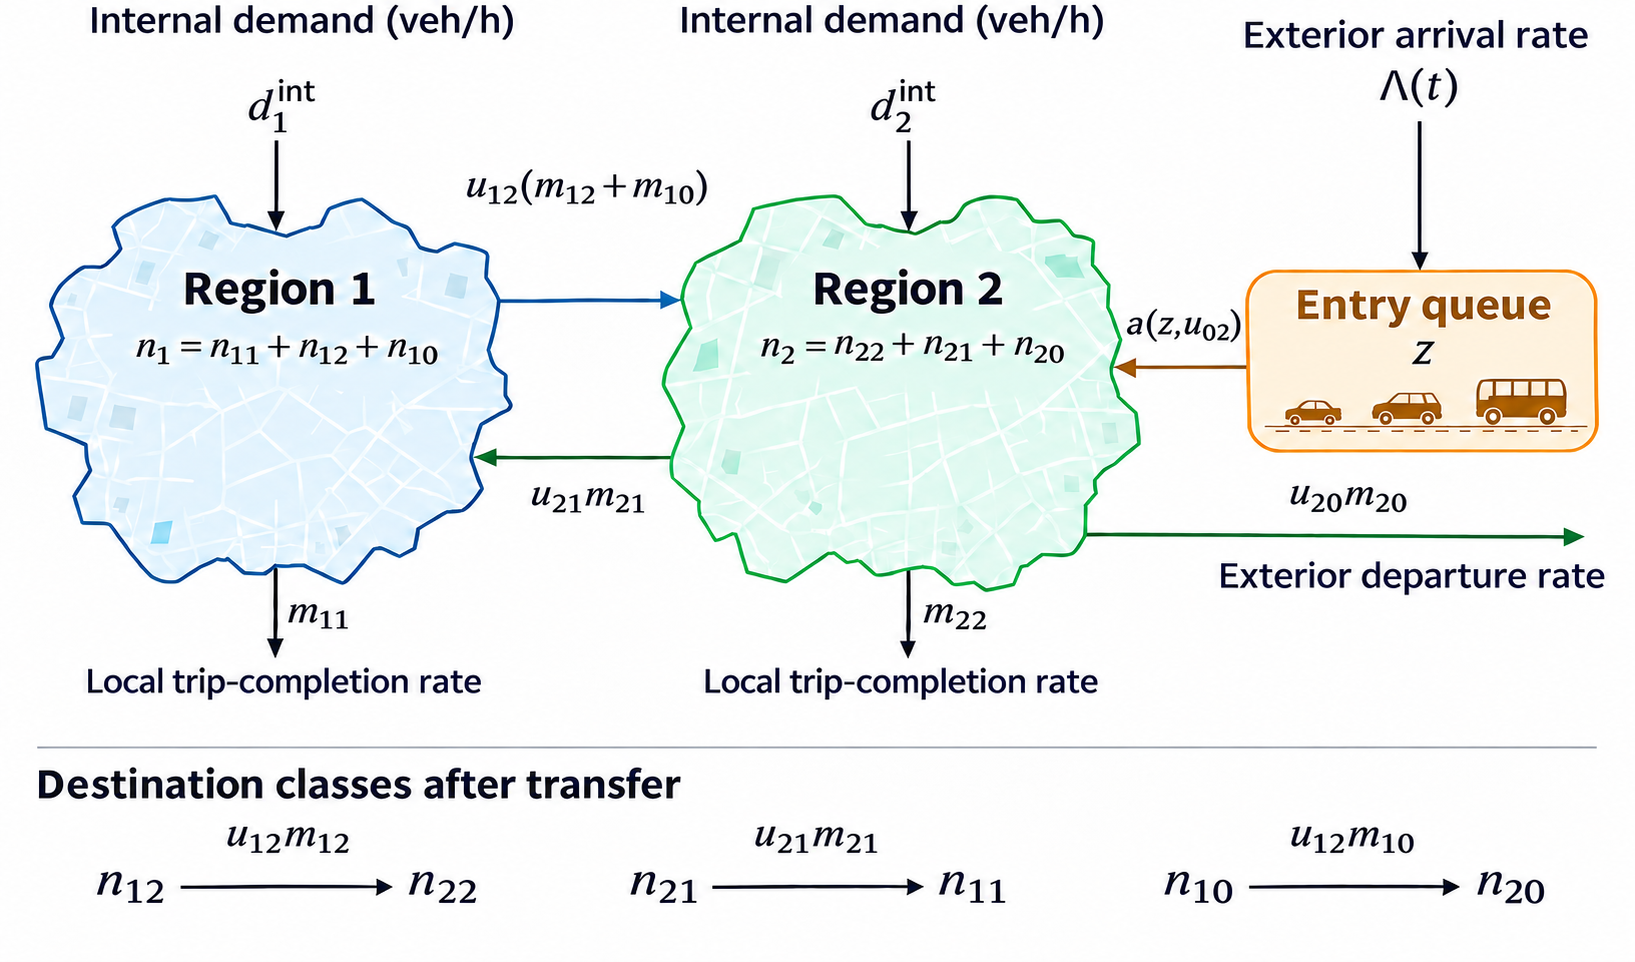
\includegraphics[width=0.98\textwidth]{figures/two_region_vehicle_flows_revised.png}
\caption{Two-region traffic model. The upper diagram shows regional
accumulations $n_1,n_2$ and the exterior entry queue $z$, all in vehicles.
Arrows show flow rates in veh/h. Here $d_i^{\rm int}$ is the total
internal demand in region $i$, $\Lambda$ is the exterior
arrival rate, and $a(z,u_{02})$ is admission to Region~2 under entrance input $u_{02}$. The perimeter control
input $u_{ij}$ regulates the boundary from $i$ to $j$, with $0$ denoting
the exterior. Potential class flows $m_{ij}$ are defined in
\eqref{eq:class-potential-flow}. Local completions are $m_{11},m_{22}$,
and $u_{20}m_{20}$ leaves the network. Fractions $\pi$ and $1-\pi$ of
admission join $n_{21}$ and $n_{22}$. The lower strip shows transfers
that change a vehicle's current region while preserving its destination.
Region shapes, streets, and vehicle icons are schematic.}
\label{fig:two-region-network}
\end{figure}

The regional totals are
\begin{equation}
 n_1=n_{11}+n_{12}+n_{10},\qquad
 n_2=n_{22}+n_{21}+n_{20}.
 \label{eq:regional-class-totals}
\end{equation}
The model treats these vehicle counts as continuous aggregate quantities.
Control inputs may switch between plan blocks, while the accumulations
remain continuous in time. A notation list is provided in
\appref{app:notation}.

For later expressions, define the potential class flow
\begin{equation}
 m_{ij}(t)=\frac{n_{ij}(t)}{n_i(t)}G_i(n_i(t)),\qquad n_i(t)>0.
 \label{eq:class-potential-flow}
\end{equation}
This is the trip-completion rate for $j=i$ and the potential transfer
rate otherwise. The allocation follows the standard MFD assumptions
\cite{geroliminis2013mpc,mohajerpoor2020hinf}:
\begin{enumerate}
\item Vehicles with destinations inside their current region complete
their trips locally. Within-region trip lengths are comparable across
destination classes and remain fixed.
\item Each destination class contributes to the MFD outflow in proportion
to its share of the regional accumulation.
\item Receiving regions can accommodate the modeled transfers. A separate
downstream receiving-supply restriction is not included.
\end{enumerate}
The two-region model uses the same fixed MFD in both regions,
$G_1=G_2=G$. Its coefficients are specified in
Section~\ref{sec:experimental-setup}. For computation, write
$m_{ij}=n_{ij}v(n_i)$, where the per-vehicle outflow rate $v$ (h$^{-1}$)
is $v(n)=G(n)/n$ for $n>0$ and
$v(0)=G'(0)$. This extension is continuous for the fitted differentiable
MFD with $G(0)=0$ and gives zero class flow at an empty region.

For interregional transfers and network departures, each control input
specifies the proportion of potential flow permitted to pass. Thus
$u=1$ permits the full potential flow and $u=0$ blocks that movement.
The entrance input $u_{02}$ instead sets the admission capacity. With
queue-release time $\tau_q>0$ and full entrance capacity $\kappa_{02}>0$,
\begin{equation}
 a(z,u_{02})=\min\{z/\tau_q,\kappa_{02}u_{02}\}.
 \label{eq:new-admission}
\end{equation}
The term $z/\tau_q$ limits admission according to the vehicles waiting,
while $\kappa_{02}u_{02}$ limits it according to the permitted capacity.
The queue is an aggregate point queue with a finite storage limit.
Its spatial extent and spillback into upstream roads are not modeled.
Explicit boundary-queue models provide a related treatment of storage
constraints \cite{haddad2017queues}, although here the queue is outside
Region~2 rather than between the two regions.

\subsection{State representation and physical constraints}
\label{sec:physical-constraints}

A control plan $P$ specifies control inputs or feedback laws over
$[t_0,E]$, from activation at $t_0$ to expiry at $E$. Section~\ref{sec:control-plans}
defines their blockwise representation. To express the model in the
coordinates used for certification, set
$d_1^{\rm int}=d_{11}^{\rm int}+d_{12}^{\rm int}+d_{10}^{\rm int}$ and
$d_2^{\rm int}=d_{22}^{\rm int}+d_{21}^{\rm int}+d_{20}^{\rm int}$.
Summing the class balances gives
\begin{equation}
\begin{aligned}
\dot n_1&=d_1^{\rm int}-m_{11}-u_{12}(m_{12}+m_{10})+u_{21}m_{21},\\
\dot n_2&=d_2^{\rm int}-m_{22}+u_{12}(m_{12}+m_{10})-u_{21}m_{21}
             +a-u_{20}m_{20}.
\end{aligned}
\label{eq:regional-flow-balances}
\end{equation}
Collect the regional totals, four destination classes, and queue as
\begin{equation}
\begin{aligned}
x&=(n_1,n_2,n_{11},n_{22},n_{10},n_{20},z)^\top,\\
u&=(u_{12},u_{21},u_{02},u_{20})^\top.
\end{aligned}
\label{eq:new-state}
\end{equation}
The other two classes are recovered exactly as
$n_{12}=n_1-n_{11}-n_{10}$ and $n_{21}=n_2-n_{22}-n_{20}$.
These coordinates therefore describe the same seven vehicle counts as
\eqref{eq:destination-class-balances}. The dynamics become
\begin{equation}
 \dot x=f(x,u,t)+e_7w(t),\qquad e_7=(0,0,0,0,0,0,1)^\top,
 \label{eq:new-plant}
\end{equation}
where $f$ contains the nominal balances with $w=0$, ordered as in
\eqref{eq:new-state}. Substituting a plan's feedback law into $f$ gives
the block dynamics $f_b$ used in the certification check.

Every plan must satisfy $u(t)\in\mathcal U$ throughout its execution,
where
\begin{equation}
\mathcal U=\{u:0\le u\le1,\ |u_{21}-u_{12}|\le\delta_1^u,
\ |u_{20}-u_{02}|\le\delta_2^u\}.
\label{eq:new-gates}
\end{equation}
The difference bounds follow Mohajerpoor et al.~\cite{mohajerpoor2020hinf}. Opposite-direction
movements can share signal phases, which motivates restricting how far
their aggregate control inputs can differ. The parameters
$\delta_1^u,\delta_2^u\in[0,1]$ specify these operating limits. Each input has the componentwise bounds $[0,1]$, in addition to these
pairwise restrictions. Minimum and maximum green-time bounds, as in
\cite{mohajerpoor2020hinf}, would tighten the componentwise range and
can be represented by the same affine constraints.

Physical feasibility also requires nonnegative destination-class
accumulations and
\[
0\le n_i\le n_i^{\max}\quad(i=1,2),\qquad 0\le z\le z^{\max}.
\]
The regional bounds are operational accumulation limits, and $z^{\max}$
is exterior storage capacity. Together with \eqref{eq:new-gates}, the
implemented two-region formulation has 24 affine state--input
inequalities. Their numerical limits are given with the experiments.

\subsection{Control objectives and service requirements}
\label{sec:benchmark-formulation}

Control objectives specify the traffic improvement sought from a plan.
The network-efficiency objective minimizes total time spent in both
regions and the exterior queue. For total accumulation
$M=n_1+n_2+z$, its cost is
\begin{equation}
J_Q(P;x_0,w)=\int_{t_0}^{E}M_P(t;x_0,w)\,dt.
\label{eq:benchmark-queue-cost}
\end{equation}
Here $x_0$ is the activation state, $w$ is the arrival error, and the
subscript $P$ denotes the trajectory generated by the plan. Costs are
measured in vehicle-hours. We suppress $x_0,w$ when they are fixed or
specified by the planning scenario.

A temporary priority for Region~2 is represented by a weight $p\ge1$:
\begin{equation}
J_D(P;x_0,w)=\int_{t_0}^{E}
 \bigl(n_{1,P}(t)+p n_{2,P}(t)+z_P(t)\bigr)\,dt.
\label{eq:benchmark-priority-cost}
\end{equation}
The trajectory components in this expression share the same $x_0,w$.
These objectives express preferences, while service requirements impose
mandatory traffic conditions at specified deadlines:
\begin{equation}
g_r^\top x(T_r)\le\eta_r,\qquad T_r\in[t_0,E].
\label{eq:new-service}
\end{equation}
The dimensionless coefficients $g_r$ select the traffic quantity,
$\eta_r$ is its limit in vehicles, and $T_r$ is its deadline. For example,
$g_r=e_1$, with $e_1$ selecting the first state component, imposes a
Region-1 accumulation limit. Service requirements
remain binding when regional priorities change. Modifying a target or
deadline requires an operator instruction.

The experiments consider a network-efficiency task that minimizes $J_Q$
subject to physical constraints, and a regional-priority task that
minimizes $J_D$ while also requiring $n_1(E)\le\eta$. The cost subscripts Q and D identify the network-efficiency and
regional-priority tasks, respectively. The next subsection specifies the uncertainty under
which their constraints must hold.

\subsection{Uncertainty and feasible plans}
\label{sec:problem-uncertainty}

At activation, the framework receives a state estimate
$\widehat x_{t_0}$ and a componentwise state-estimation error bound
$d_x\in\mathbb R_{\ge0}^7$ in vehicles. The bound holds simultaneously
for all components. The resulting box is
\begin{equation}
\begin{aligned}
\mathcal I_{t_0}&=\{x:|x-\widehat x_{t_0}|\le d_x\},\\
|w(t)|&\le\bar w,\qquad t\in[t_0,E],
\end{aligned}
\label{eq:benchmark-contract}
\end{equation}
where inequalities are componentwise and $\bar w$ is in veh/h.
The vector $d_x$ gives the box's \emph{half-widths}, meaning its distances
from the center to each face. Measurement processing and state estimation
supply the initial estimate and bound externally. Numerical sweeps use a
scalar parameter $d$ to construct $d_x$ as specified for each study.
The forecast $\widehat\Lambda$ and error bound are chosen so that all
allowed arrivals are nonnegative. Later decisions use a fresh bounded
estimate or a propagated certified state set, as described in
Section~\ref{sec:new-execution}.
\begin{definition}
\label{def:planning-contract}
The \emph{planning contract} is the tuple
\[
\mathcal C=(\mathcal I_{t_0},\bar w,f,\mathcal P_{\rm phys},
\mathcal O,[t_0,E]).
\]
Here $f$ includes the arrival forecast, $\mathcal P_{\rm phys}$ contains
the physical constraints, and $\mathcal O$ contains the service triples
$(T_r,g_r,\eta_r)$ to be met during the execution interval.
\end{definition}
Let $\mathcal W$ contain every measurable arrival error satisfying
\eqref{eq:benchmark-contract}. Write $x_P(s;x_0,w)$ and $u_P(s;x_0,w)$
for the state and applied control at time $s$ under plan $P$.

\begin{definition}
\label{def:robust-feasibility}
Write the physical constraints as $H_jx+J_ju\le\beta_j^{\rm phys}$ and
the service requirements as $g_r^\top x(T_r)\le\eta_r$.
A robustly feasible plan has a well-defined trajectory throughout
$[t_0,E]$ for every allowed initial state and arrival error, and satisfies
all physical constraints throughout this interval and all service
requirements at their deadlines. The set of these plans is
\begin{equation}
\begin{aligned}
\mathcal F_{\mathcal C}=\{P:\;&\forall x_0\in\mathcal I_{t_0},\ w\in\mathcal W,\\
&H_jx_P(s;x_0,w)+J_ju_P(s;x_0,w)\le\beta_j^{\rm phys}\\
&\hspace{1em}\text{for all }s\in[t_0,E]\text{ and physical constraints }j,\\
&g_r^\top x_P(T_r;x_0,w)\le\eta_r
\quad\text{for all service requirements }r\}.
\end{aligned}
\label{eq:benchmark-feasible-set}
\end{equation}
\end{definition}

\begin{definition}
\label{def:feasibility-certificate}
A certification check must accept only robustly feasible plans:
\[
\mathsf{Cert}_{t_0}(P\mid\mathcal C)=1
\quad\Longrightarrow\quad P\in\mathcal F_{\mathcal C}.
\]
Its accepted set therefore satisfies
\begin{equation}
\widehat{\mathcal F}_{\mathcal C}
=\{P:\mathsf{Cert}_{t_0}(P\mid\mathcal C)=1\}
\subseteq\mathcal F_{\mathcal C}.
\label{eq:benchmark-certifiable-set}
\end{equation}
\end{definition}
Theorem~\ref{thm:new-plan-enclosure} and
Proposition~\ref{prop:structure-plan} establish this property for the
checks constructed in Section~\ref{sec:new-certification}. An
inconclusive check leaves feasibility undecided. A demonstrated
violation in any allowed realization establishes robust infeasibility.

\begin{problem}
\label{prob:supervised-planning}
Consider model~\eqref{eq:new-plant}, a planning contract $\mathcal C$,
and plans proposed at successive request times.
\begin{enumerate}
\item Construct a computable certification procedure satisfying
Definition~\ref{def:feasibility-certificate} and an activation rule that
permits replacement only when a matching certificate is completed by
the activation time.
\item When a proposal is not certified, seek a modified plan that passes
the same check, using a backup certified for the applicable contract.
If no replacement is ready in time, continue the current plan under
its existing certificate.
\item Across successive requests and computation delays, activate a
replacement only when its certificate covers every possible activation
state and every pending service requirement. Otherwise retain
the current plan within its original execution interval.
\end{enumerate}
\end{problem}
Planning tools seek low cost under forecast or scenario conditions.
Certification checks feasibility over the whole uncertainty set, and a
failed check may be inconclusive.

\section{Dual-Agent Planning and Supervisory Control}
\label{sec:new-agent}

\subsection{Architecture overview}

Figure~\ref{fig:new-architecture} shows the architecture. The AI agent
interprets operator instructions and requests plans from planning tools.
The rule-based supervisory agent, called the \emph{supervisor} below,
checks candidate plans and authorizes execution only when their
certificates match the activation conditions. Traffic information,
physical constraints, and service requirements reach the tools and supervisor
independently of the AI agent. The guarantee therefore does not depend
on the agent's interpretation or memory being correct.

Hierarchical perimeter control coordinates control decisions across
levels \cite{ramezani2015heterogeneity,su2023hierarchical}, whereas the
proposed architecture separates plan proposal from the verification
required before execution. The same interface can receive plans from
a learned controller, a numerical optimizer, or a human operator.
The agent study in Section~\ref{sec:task-state-live} uses an LLM with
tool calling. A deterministic tool interface validates requests, invokes
the planning or repair procedure, and forwards its output to the
supervisor and agent.

\begin{figure}[!t]
\centering
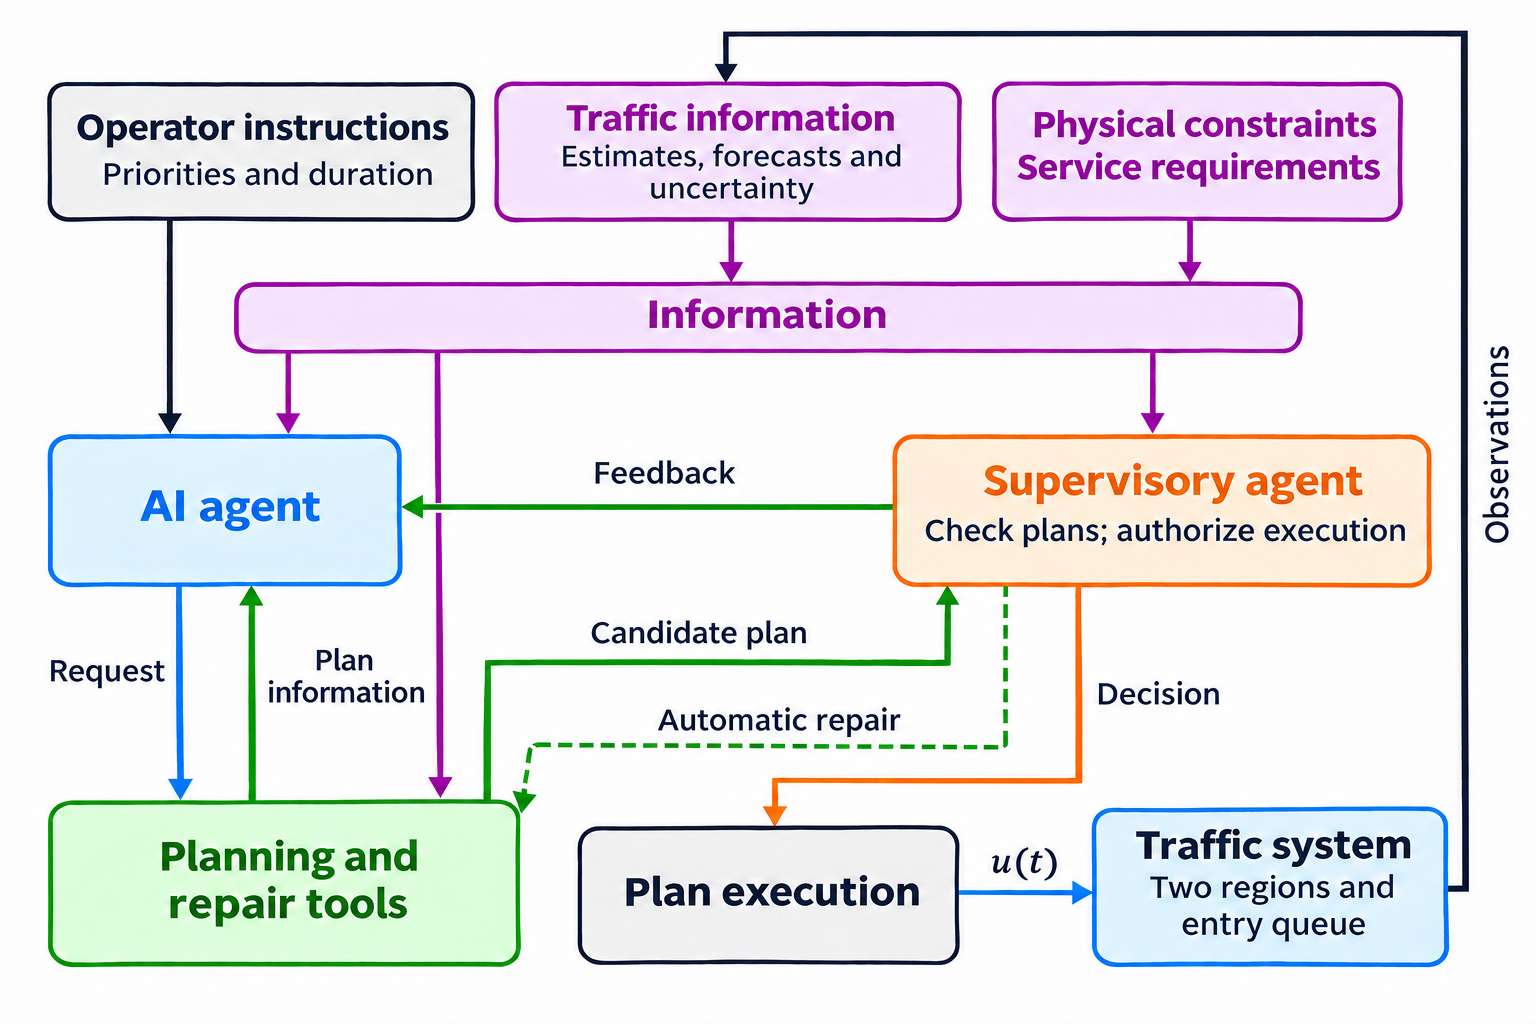
\includegraphics[width=0.98\textwidth]{figures/dual_agent_architecture_revised.png}
\caption{Planning and supervisory decisions. Traffic information and
authorized physical constraints and service requirements are supplied
independently of the AI agent. The tool interface forwards each candidate
directly to the supervisor and provides plan information and feedback to
the agent. Repair can be requested by the agent or invoked automatically
by the supervisor, depending on the configured mode. Both routes produce
candidates subject to the same check. Only the supervisor authorizes
replacement. Observations feed the external traffic-information source.
A feedback plan additionally requires the state access specified in
Section~\ref{sec:control-plans}.}
\label{fig:new-architecture}
\end{figure}

\subsection{Control plans}
\label{sec:control-plans}

A plan specifies the control law and its timing over a finite interval:
\begin{equation}
\begin{aligned}
P&=\bigl((\tau_b,\tau_{b+1},k_b,K_b)\bigr)_{b=0}^{N_b-1},
\qquad t_0=\tau_0<\cdots<\tau_{N_b}=E,\\
u_P(t)&=k_b+K_bx(t),\qquad t\in[\tau_b,\tau_{b+1}).
\end{aligned}
\label{eq:control-plan-tuple}
\end{equation}
Here $N_b$ is the number of control blocks and $E$ is the plan expiry.
The last block supplies the left-limit value at $E$ unless a certified
successor starts there. State trajectories remain continuous when the
input changes, and the certificate checks the applicable constraints on
both sides of each change.

For feedback around a target $x_b^\star$ and reference input $u_b^\star$,
$k_b=u_b^\star-K_bx_b^\star$ gives
$u=u_b^\star+K_b(x-x_b^\star)$. When $K_b\ne0$, the execution model
assumes that this law uses the true state $x(t)$. Uncertainty in the
activation state is still allowed: certification covers every trajectory
starting in the supplied set and following this feedback law. Applying
the law to an estimate during execution would additionally require bounds
on the resulting input error.

For $K_b=0$, a plan is an open-loop, piecewise-constant schedule. A model
predictive control (MPC) planning tool can generate such a schedule by
finite-horizon optimization. The tool solves at planning requests, and
the resulting schedule runs until expiry or a certified replacement.
Thus a new optimization enters execution through the supervisory rule
described below.

A plan specifies control inputs over the finite execution interval
$[t_0,E]$. Its certificate checks those inputs against the model,
uncertainty bounds, and service requirements over the same interval.
The expiry $E$ therefore marks the end of the period covered by this
guarantee. To maintain the guarantee after $E$, a certified replacement
must be ready by then, or execution must switch to a terminal policy
whose conditions have already been verified. \appref{sec:terminal-backup}
gives sufficient conditions for this second option.

\subsection{AI agent and planning tools}
\label{sec:agent-requests}

At request time $t_i^{\rm req}$, the agent receives the operator's
instruction, summaries of traffic information and authorized requirements,
and its interaction history. The history consists of earlier instructions,
tool responses, and supervisory feedback. Memory is a stored summary of
that history supplied to later requests. A planning tool is a callable
numerical procedure that returns a candidate plan for a specified
objective. A repair tool searches for a modified candidate after a failed
check.

The history-only agent-input format provides these instructions and
history directly. The task-record format additionally provides
$\theta_i$, which stores the active priority, its absolute expiry
$T^{\rm prio}$, and interrupted priorities. Set, Interrupt, Continue,
Extend, Resume, and Cancel update this record according to
Table~\ref{tab:task-operations} in \appref{app:task-operations}.
Priority expiries are absolute times, so an interrupted priority continues
to age. Section~\ref{sec:task-state-live} compares the two input formats.

The request compiler $\mathsf{Comp}$ is the deterministic procedure that
validates an operation, updates $\theta_i$, and converts the result into
the numerical request $q_i^A$. This request identifies the objective,
its remaining priority duration, and the corresponding cost weights.
Invalid requests give $q_i^A=\bot$ and no planning call. Changes in
priority affect the objective while preserving pending service requirements.

The tool interface sends each candidate $P_i^0$ directly to the supervisor
and returns plan information and supervisory feedback to the AI agent.
The framework supports two repair modes: the supervisor can invoke repair
automatically after rejection, or the agent can request repair in response
to the feedback. Section~\ref{sec:new-incident-protocol} uses automatic
repair, while the agent planning study in
Section~\ref{sec:task-state-live} uses agent-requested repair. Both modes
apply the same certification and activation rules.

\subsection{Supervisory agent}
\label{sec:supervisory-agent}

The supervisor checks the candidate against the current traffic
information and requirements. A \emph{certificate} records the checked
plan, its contract and execution interval, and verified bounds supporting
acceptance. A certificate \emph{matches} execution when its plan
coefficients, activation time, model and data versions, and physical and
service requirements agree with those in force, and its state and arrival
sets cover the execution uncertainty.

The decision record is
\[
\mathcal S_t=(\mathcal I_t,\mathcal W_t,\mathcal O_t,
P_t^{\rm cur},\mathcal H_t,P_t^B,t,\mathsf v_t).
\]
Here $\mathcal I_t$ is the supplied or propagated state set,
$\mathcal W_t$ is the allowed arrival-error family, and $\mathcal O_t$
contains \emph{pending service requirements}: accepted requirements whose
deadlines have not passed. The current plan $P_t^{\rm cur}$ executes
under the certificate stored in $\mathcal H_t$, which retains its
original conditions, expiry $E_{\rm cur}$, and reachable sets with their
shared uncertainty dependence. The identifier $\mathsf v_t$ records the
versions of the model, forecast, physical constraints, and service
requirements. A task-version change means that the authorized requirements
or their deadlines have changed. A backup $P_t^B$ is recorded when
available for repair under the current contract, with $P_t^B=\bot$ when
none is available.

For a candidate with activation time $t$ and expiry $E$, these fields
specify the contract $\mathcal C(\mathcal S_t,E)$ of
Definition~\ref{def:planning-contract}. Thus
$\mathsf{Cert}_t(P\mid\mathcal S_t)$ denotes the same check as
$\mathsf{Cert}_t(P\mid\mathcal C(\mathcal S_t,E))$. It checks the exact
candidate against the state set, model, uncertainty, physical constraints,
and pending requirements applicable to its execution interval.

If the original proposal passes and its certificate is ready by
activation, the supervisor may activate it unchanged. Otherwise, repair
may seek a passing alternative. If no candidate has a matching
certificate ready in time, the current plan continues under its original
certificate through $E_{\rm cur}$. When repair is invoked, the call is
\begin{equation}
\widehat P_i^R=\mathsf{RepairTool}
(P_i^0,P_i^B,\mathcal S_{t_i},\mathcal G_{\rm rep}).
\label{eq:repair-tool-interface}
\end{equation}
The backup $P_i^B$ must be certified under the same conditions as the
repair candidates. It can be the remaining current plan, rechecked for
those conditions, or a newly constructed certified backup. The output
$\widehat P_i^R$ must pass the same check before activation.
Section~\ref{sec:predictive-repair} gives the finite-grid search.
The backup is distinct from the terminal policy for operation beyond
plan expiry.

\begin{remark}
Failure to recertify the current plan from an enlarged state set does
not invalidate its original certificate. If its original assumptions
continue to hold, execution can retain the original schedule and
certificate, including its stored uncertainty dependencies, until expiry
or a later certified replacement.
\end{remark}

\subsection{Timing, assumptions, and execution}
\label{sec:execution-interface}

The request time $t_i^{\rm req}$ precedes or equals the decision time
$t_i$, at which a replacement may activate. In the planning and execution
notation, $i$ indexes decisions in $t_i$, $\mathcal I_i$,
$\mathcal S_{t_i}$, $P_i$, $\theta_i$, and $q_i^A$, with
$\mathcal I_i=\mathcal I_{t_i}$. Regional and boundary
indices in $n$, $G$, $m$, $d^{\rm int}$, and $u$ retain their traffic
meaning. We write $t_{\rm ready}$ for the time at which a candidate
certificate is complete. Planning requests and control-block changes
occur at discrete times within the continuous traffic evolution.
Computation does not shift accepted service deadlines. Only finitely many
plan decisions are allowed in any finite time interval.
Figure~\ref{fig:activation-timeline} illustrates these distinct times.

The first assumption specifies the external information on which
certification depends.

\begin{assumption}
\label{ass:trusted-inputs}
Each externally supplied state set contains the actual state at its
timestamp, the stated arrival-error bounds hold, and traffic follows
\eqref{eq:new-plant} under the model and uncertainty assumptions of the
active certificate. Physical constraints and service requirements are
authorized by the operator. These data reach the tools and supervisor
independently of agent requests and memory.
\end{assumption}

The second assumption specifies the integrity of the execution interface.

\begin{assumption}
\label{ass:supervisory-separation}
The execution interface satisfies the following conditions:
\begin{enumerate}
\renewcommand{\labelenumi}{(\alph{enumi})}
\item Agent outputs cannot modify independently supplied data, pending
requirements, or the decision record.
\item Only the supervisor authorizes activation, and execution uses the
checked coefficients, timing, and model version.
\item A new service requirement becomes pending only when the selected
plan covers it.
\item Invalid requests, failed checks, and late results leave the current
plan and its original certificate in use, while their assumptions hold,
until expiry or a later certified replacement.
\end{enumerate}
\end{assumption}

Corollary~\ref{cor:agent-independent-execution} uses both assumptions.
The guarantee concerns the feasibility of whichever candidate the
supervisor receives. The agent's interpretation of the requested objective
is evaluated separately.

\begin{figure}[!htbp]
\centering
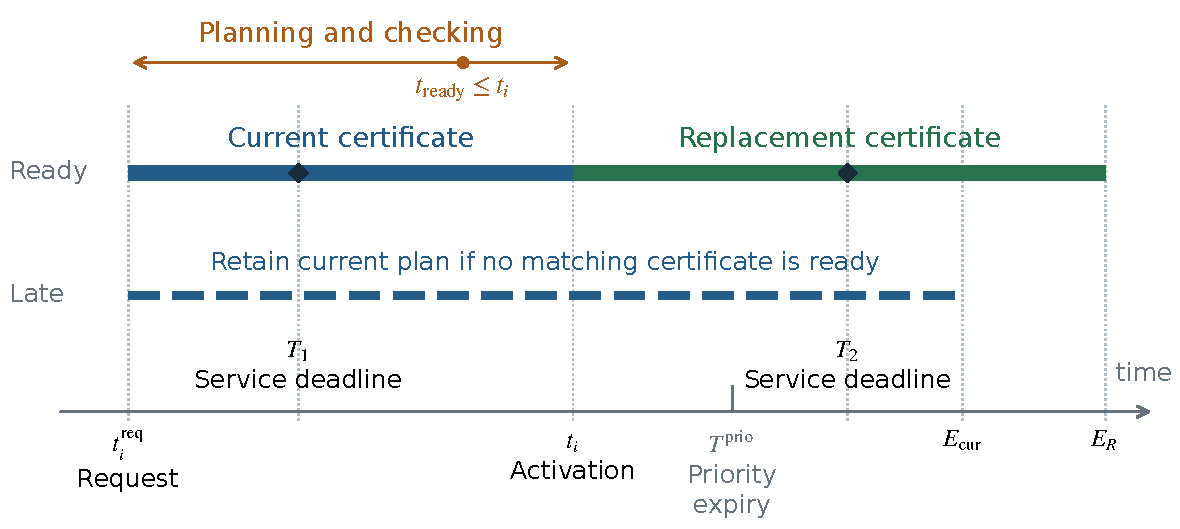
\includegraphics[width=\textwidth]{figures/certified_activation_timeline.pdf}
\caption{Example of delayed activation in
Proposition~\ref{prop:planned-handover}. The current certificate covers
execution and the service deadline $T_1$ during computation. A replacement
ready by $t_i$ and certified from a containing activation-state set covers
the later deadline $T_2$ through its expiry $E_R$. If no matching
certificate is ready, the current plan remains in force under its
original conditions, through $E_{\rm cur}$. The priority expiry $T^{\rm prio}$
and service deadlines have no fixed position relative to activation.
The ordering shown is illustrative and assumes no further replacement.}
\label{fig:activation-timeline}
\end{figure}

\begin{algorithm}[!htbp]
\caption{Planning requests and certified execution}
\label{alg:agent-execution}
\begin{minipage}{\linewidth}
\small
\textbf{Input:} current certified plan and decision record
$\mathcal S_t$, operator requests, traffic information and authorized
requirements, agent history, and task record $\theta_i$ when used.\\
\textbf{Output:} the plan selected for execution and its matching
certificate, updated decision record, and agent feedback.\\
For each request at $t_i^{\rm req}$, execute the following steps while
the current plan continues within its execution interval.
\begin{enumerate}
\setlength{\itemsep}{2pt}
\item \label{step:request}\textbf{Interface and AI agent:}
process priority expiries and obtain a planning request. In the task-record
variant, apply $\mathsf{Comp}$ to validate the requested operation and
form $q_i^A$. Otherwise validate the directly supplied planning request.
If $q_i^A=\bot$, retain the current record and return feedback.
\item \label{step:planning}\textbf{Planning tool and interface:}
use $q_i^A$ and independently supplied data to generate $P_i^0$.
Forward the candidate directly to the supervisor and provide plan
information to the AI agent.
\item \label{step:activation}\textbf{Supervisor:}
specify $t_i\ge t_i^{\rm req}$ and assemble $\mathcal S_{t_i}$ with
a state set obtained by propagating the supplied state set under the
current plan, as in Proposition~\ref{prop:planned-handover}, or from a
valid estimate at activation. Preserve accepted deadlines, including those
during computation.
\item \label{step:checking}\textbf{Supervisor and repair tool:}
evaluate $\mathsf{Cert}_{t_i}(P_i^0\mid\mathcal S_{t_i})$ using
Theorem~\ref{thm:new-plan-enclosure}, with the optional refinements in
Proposition~\ref{prop:structure-plan}.
After rejection, invoke $\mathsf{RepairTool}$ only when requested by the
agent or enabled by the automatic repair mode. Certify each repair under
the same conditions, using a backup certified for those conditions.
\item \label{step:installation}\textbf{Supervisor:}
activate a candidate at $t_i$ only if its matching certificate is complete
by $t_i$, its execution data match, and it covers all pending
requirements. Otherwise retain the current plan, original certificate,
and expiry. Accept a new service requirement only when the selected plan
covers it.
\item \label{step:feedback}\textbf{Interface:}
return the decision to the agent, update its history and the decision
record, and continue execution within the selected plan's execution interval.
\end{enumerate}
\end{minipage}
\end{algorithm}


% Keep the architecture timeline and execution algorithm in Section 3.
\FloatBarrier
\section{Runtime Certification Using Traffic Structure}
\label{sec:new-certification}


We first certify a single plan, then use its certificate to justify
replacement, repair, and delayed activation. Conservation coordinates
preserve the shared effect of admission on queues and destination classes.
Nonnegativity, scalar queue comparison, and signed uncertainty propagation
provide tighter bounds within these coordinates. The final subsection
extends the construction to several entry queues. These results cover
each selected plan over its execution interval. \appref{sec:terminal-backup}
gives sufficient conditions and proofs for maintaining the guarantees
beyond that interval, using a terminal policy and an invariant set that
also cover pending service requirements. \appref{sec:repair-cost-bound}
provides a conditional bound on the traffic cost of repair. The numerical
studies evaluate finite plans and report their measured repair costs.

The enclosure arguments use validated numerical bounds
\cite{tucker2011validated}, generalized Jacobians for the admission
minimum \cite{clarke1990optimization}, and scalar and componentwise
comparison \cite{khalil2002nonlinear,farina2000positive}.
The complete proofs below specify how these tools apply to the traffic
model and its execution rules.

\subsection{Plan data and conservation coordinates}

For each block of a plan defined in Section~\ref{sec:control-plans},
the certification procedure uses the control law and arrival uncertainty
\begin{equation}
 u_b(x)=k_b+K_bx,
 \qquad \Lambda(t)=\widehat\Lambda(t)+w(t),
 \qquad |w(t)|\le\bar w.
 \label{eq:new-plan-data}
\end{equation}
The primary two-region forecast is continuous and piecewise affine.
The arrival error $w$ may be any measurable signal within this bound.
For $K_b\ne0$, the exact-state feedback assumption in
Section~\ref{sec:control-plans} applies. Bounds on the effects of
measurement errors are needed when implementing feedback from estimates.

For the physical constraints in Definition~\ref{def:robust-feasibility},
substitution of the block law gives
\begin{equation}
 h_{jb}^\top x\le\beta_{jb},\qquad
 h_{jb}^\top=H_j+J_jK_b,\qquad
 \beta_{jb}=\beta_j^{\rm phys}-J_jk_b.
 \label{eq:new-physical-rows}
\end{equation}
Here $j=1,\ldots,n_c$ indexes physical constraints. The service
requirements remain $g_r^\top x(T_r)\le\eta_r$ for $r=1,\ldots,n_s$,
as in \eqref{eq:new-service}. Each two-sided input-difference bound in
\eqref{eq:new-gates} contributes two physical inequalities.

The main difficulty in bounding these constraints is that admission
simultaneously decreases the exterior queue and increases the receiving
destination classes. We preserve this shared effect by combining each
class with its allocated share of the queue. For the fixed destination
fraction $\pi$, use
\begin{equation}
\begin{aligned}
y=Lx=(&n_{11},n_{12},n_{10},n_{22}+(1-\pi)z,\\
      &n_{21}+\pi z,n_{20},z)^\top.
\end{aligned}
\label{eq:new-conservation-coordinates}
\end{equation}
Admitting a vehicle transfers it from the queue into the region without
changing the corresponding combined quantity. The transformation is
invertible, with
\begin{equation}
 \begin{aligned}
 n_1&=y_1+y_2+y_3,&n_2&=y_4+y_5+y_6-y_7,\\
 n_{11}&=y_1,&n_{22}&=y_4-(1-\pi)y_7,\\
 n_{10}&=y_3,&n_{20}&=y_6,\qquad z=y_7.
 \end{aligned}
 \label{eq:new-inverse-coordinates}
\end{equation}
For admission incidence $b_a=(0,1,0,1-\pi,0,0,-1)^\top$,
\begin{equation}
 Lb_a=-e_7,
 \qquad Le_7=(0,0,0,1-\pi,\pi,0,1)^\top.
 \label{eq:new-conservation-incidence}
\end{equation}
Adding each receiving-class balance to its share of
$\dot z=\Lambda-a$ cancels admission from the combined accumulations.
Consequently $n_1+n_2+z=\sum_{i=1}^6y_i$, and explicit admission remains
only in the queue equation. For example,
\[
\begin{aligned}
\frac{d}{dt}(n_{21}+\pi z)
 &=d_{21}^{\rm int}-u_{21}m_{21}+\pi\Lambda,\\
\frac{d}{dt}(n_{22}+(1-\pi)z)
 &=d_{22}^{\rm int}-m_{22}+u_{12}m_{12}+(1-\pi)\Lambda.
\end{aligned}
\]
Bounding the class and queue separately can count the same uncertain
admission twice with opposite signs. These combined balances cancel it
before bounding. Regional MFD outflow still depends on the full
transformed state, and the independent queue equation remains necessary
to recover regional accumulations and verify storage.

\subsection{Certification of one plan}
\label{app:new-enclosure-proof}

Let $f_b(x,t)$ denote the traffic-state rate of change under control
block $b$ and the nominal arrival forecast. The actual rate of change is
$f_b(x,t)+e_7w(t)$. Class flows use the per-vehicle outflow rate $v$ defined in
Section~\ref{app:new-model}.
The admission minimum has affine branches under affine feedback. Their
minimum is continuous and locally Lipschitz, so the field is locally
Lipschitz in state and measurable in time. Bounded measurable arrival errors
therefore give unique local absolutely continuous solutions. The compact enclosures constructed below bound these solutions and allow
them to continue throughout each finite plan. An enclosure is a computed
set guaranteed to contain every traffic state allowed by the initial
information and uncertainty assumptions.

The certification procedure partitions the plan at control-block changes, forecast-slope
changes, service deadlines, and prediction checkpoints. On each interval
$[t_l,t_l+h_l]$, a differentiable curve $\mathbf p_l$ predicts the nominal
state. The implementation uses a local quadratic predictor constructed
from the nominal field, its Jacobian, and the forecast slope. It need not
solve the dynamics exactly: the derivative mismatch is bounded below.
Inherited radii $r_l\ge0$ satisfy
$|L(x(t_l)-\mathbf{p}_l(t_l))|\le r_l$. For an initial physical box centered at
$\mathbf{p}(t_0)$ with half-width $d_x$, use $r_0\ge|L|d_x$. The initial predictor
box is $\mathbf{p}(t_0)+L^{-1}[-r_0,r_0]$. A trial radius $R_l>0$ defines
$\mathbf{p}_l(t)+L^{-1}[-R_l,R_l]$, a proposed region around the predictor in which
we seek to contain the traffic state throughout the interval. This moving
region is an a priori enclosure, also called a trial tube. The checks
below establish containment of every allowed trajectory. On this whole
region and time interval, obtain
\begin{equation}
 \begin{aligned}
 a_{il}&\ge\sup (L D_xf_b L^{-1})_{ii},\\
 b_{ijl}&\ge\sup |(L D_xf_b L^{-1})_{ij}|\quad(j\ne i),\\
 \delta_{il}&\ge\sup_t |(L f_b(\mathbf{p}_l(t),t)-L\dot{\mathbf{p}}_l(t))_i|.
 \end{aligned}
 \label{eq:new-local-bounds}
\end{equation}
A branch surface is where the expression determining the minimum
admission flow changes. At such a surface the generalized Jacobian is
contained in the convex
hull of limiting smooth branch Jacobians. Both branches are included
whenever the trial region meets that surface. A branch is omitted only
when verified bounds exclude it throughout the region. The diagonal bound
retains its sign, while cross-component terms use magnitudes.

The scalar comparison is
\begin{align}
 c_{il}(R_l)&=\sum_{j\ne i}b_{ijl}R_{jl}
                  +\delta_{il}+|(Le_7)_i|\bar w,\nonumber\\
 \phi_{il}(s)&=e^{a_{il}s}r_{il}
                   +\chi(a_{il},s)c_{il}(R_l),\nonumber\\
 \chi(a,s)&=\begin{cases}(e^{as}-1)/a,&a\ne0,\\s,&a=0.\end{cases}
 \label{eq:new-component-comparison}
\end{align}
Containment and continuous physical feasibility pass when
\begin{align}
 \max\{r_{il},\phi_{il}(h_l)\}&<R_{il}\quad\text{for every }i,
 \label{eq:new-self-inclusion}\\
 \sup_{t\in[t_l,t_l+h_l]}h_{jb}^\top \mathbf{p}_l(t)
       +|h_{jb}^\top L^{-1}|R_l&\le\beta_{jb}.
 \label{eq:new-affine-support}
\end{align}
The first inequality is a self-inclusion check: the computed error bounds
remain strictly inside the trial region used to derive them. The second
checks physical constraints at every time in that interval. Absolute values
are componentwise. When moving to the next interval, account for any
change in the predictor's center by
\begin{equation}
 \delta^{\rm rec}_l\ge
 |L(\mathbf{p}_l(t_{l+1})-\mathbf{p}_{l+1}(t_{l+1}))|,
 \label{eq:new-recentering-bound}
\end{equation}
and propagate $r_{i,l+1}=\phi_{il}(h_l)+\delta^{\rm rec}_{il}$. At a service checkpoint, the paired predictor center $\mathbf p(T_r)$
and inherited radius $r(T_r)$ give
\begin{equation}
 g_r^\top\mathbf p(T_r)+|g_r^\top L^{-1}|r(T_r)\le\eta_r.
 \label{eq:new-service-support}
\end{equation}

At control or target changes, propagate the inherited box and check
the successor input constraints on it. The following theorem then
establishes the certified-set containment in
\eqref{eq:benchmark-certifiable-set} for every trajectory allowed by
the plan's initial set and uncertainty bounds.

\begin{theorem}
\label{thm:new-plan-enclosure}
Consider the MFD field \eqref{eq:new-plant} with admission
\eqref{eq:new-admission}, a finite affine-feedback plan implemented as
$u(t)=u_b(x(t))$, and the uncertainty
class \eqref{eq:new-plan-data}. Let its initial information set be contained
in the initial predictor box. Suppose the bounds
\eqref{eq:new-local-bounds} hold for every state and time in each trial
region, and
\eqref{eq:new-self-inclusion} holds on every interval. Then the propagated
boxes contain every trajectory from that initial set under every allowed
arrival error. If \eqref{eq:new-affine-support} and
\eqref{eq:new-service-support} also pass, the trajectory satisfies every
physical constraint continuously through the plan's expiry and every included
service requirement at its deadline, including the successor-input
constraints checked at block boundaries.
\end{theorem}

\begin{proof}
Consider one interval $[t_l,t_l+h]$ and omit its index from the bounds.
Define $z_e=L(x-\mathbf p)$. Initially $|z_e(t_l)|\le r<R$.
Before any $|(z_e)_i|$ first reaches $R_i$, the segment from the predictor
to the true state lies in the trial region. The locally Lipschitz
mean-value relation \cite{clarke1990optimization} gives, almost everywhere,
\begin{equation}
 \dot z_e=A(t)z_e+\epsilon(t)+(Le_7)w(t),
 \label{eq:new-error-dynamics}
\end{equation}
where $\epsilon=Lf_b(\mathbf p,t)-L\dot{\mathbf p}$ and
$|\epsilon_i|\le\delta_i$. The matrix $A(t)$ is a weighted average of
transformed generalized Jacobians along that segment. Its nonnegative
weights sum to one, so the branch bounds also give
$A_{ii}\le a_i$ and $|A_{ij}|\le b_{ij}$ for $j\ne i$.

For $v_i=|(z_e)_i|$, the cross-component bounds $v_j\le R_j$ imply
\begin{equation}
 \dot v_i\le a_iv_i+c_i(R)
 \quad\text{almost everywhere before boundary contact}.
 \label{eq:new-error-comparison-proof}
\end{equation}
This inequality also holds almost everywhere at zero components.
Multiplication by $e^{-a_i(t-t_l)}$ and integration yield
\[
 v_i(t_l+s)\le e^{a_i s}r_i+
       \int_0^s e^{a_i(s-\tau)}c_i(R)\,d\tau=\phi_i(s).
\]
Since $\phi_i'(s)=e^{a_i s}(a_ir_i+c_i(R))$ has constant sign,
its maximum on $[0,h]$ is $\max\{r_i,\phi_i(h)\}<R_i$ by
\eqref{eq:new-self-inclusion}. Continuity makes this strict bound
incompatible with a first boundary contact. The bounded enclosure and
local regularity also allow the solution to continue to the endpoint.

At $t_{l+1}$, the old-center error is bounded by $\phi(h)$. Physical
states are continuous across control-input changes, so the triangle inequality
and \eqref{eq:new-recentering-bound} give
\[
 |L(x(t_{l+1})-\mathbf p_{l+1}(t_{l+1}))|
 \le\phi(h)+\delta_l^{\rm rec}=r_{l+1}.
\]
Induction over the finite partition proves containment. For a physical
constraint, substitution of $x=\mathbf p+L^{-1}z_e$ gives
$h_{jb}^\top x\le h_{jb}^\top\mathbf p+|h_{jb}^\top L^{-1}|R$.
Its time maximum is bounded by \eqref{eq:new-affine-support}.
The endpoint box similarly gives
$g_r^\top x(T_r)\le g_r^\top\mathbf p(T_r)+
|g_r^\top L^{-1}|r(T_r)\le\eta_r$ by
\eqref{eq:new-service-support}. The inherited box also checks the new
control input at each boundary. Thus every physical and scheduled service
constraint holds on its specified interval or deadline.
\end{proof}


Every acceptance bound includes numerical rounding error.
\appref{app:verified-arithmetic} gives the outward-rounding rules and
exact checks for constant control inputs.

\subsection{Traffic structure and tighter bounds}
\label{sec:structure-certificate}
\label{app:structure-proof}

The preceding certificate provides a general bound, but separate bounds
on each state component can lose useful information about vehicle
conservation. For constant control inputs, three features of the traffic model
allow tighter checks of the same constraints: destination classes remain
nonnegative, the exterior queue has an independent scalar balance, and
the state errors share the same uncertain initial conditions.

\paragraph{Nonnegative destination classes}
The derived class balances are
\begin{equation}
 \begin{aligned}
 \dot n_{12}&=d^{\rm int}_{12}-u_{12}v(n_1)n_{12},\\
 \dot n_{21}&=d^{\rm int}_{21}+\pi a-u_{21}v(n_2)n_{21}.
 \end{aligned}
 \label{eq:structure-derived-classes}
\end{equation}
For a quadratic per-vehicle outflow rate
$v(n)=\alpha_2n^2+\alpha_1n+\alpha_0$, the sufficient conditions
$\alpha_2>0$ and $4\alpha_2\alpha_0-\alpha_1^2>0$ give
\begin{equation}
 v(n)=\alpha_2\left(n+\frac{\alpha_1}{2\alpha_2}\right)^2+
                    \frac{4\alpha_2\alpha_0-\alpha_1^2}{4\alpha_2}>0.
 \label{eq:structure-positive-factor}
\end{equation}
This completion-of-the-square identity establishes positivity on the
whole nonnegative domain. The fitted coefficients used in
Section~\ref{sec:experimental-setup} satisfy these inequalities.
More generally, the structural result below requires a nonnegative
per-vehicle outflow rate on its stated domain.

\paragraph{Independent queue bounds}
With constant control inputs, the queue depends on its own accumulation and
the exterior arrival rate, so it can be bounded before the coupled
regional states. It satisfies the scalar equation
\begin{equation}
 \dot z=\widehat\Lambda(t)+w(t)-\min\{z/\tau_q,\kappa_{02}u_{02}\}.
 \label{eq:structure-scalar-queue}
\end{equation}
Extreme initial queues and arrival bounds define lower and upper
comparison solutions. Write $\bar a=\kappa_{02}u_{02}$ for the constant
admission capacity set by the entrance input. For constant exterior arrival
$\Lambda_*$, each branch has the solution
\begin{equation}
 \begin{aligned}
 z(s)&=\tau_q\Lambda_*+(z_0-\tau_q\Lambda_*)e^{-s/\tau_q}
       &&(z/\tau_q\le\bar a),\\
 z(s)&=z_0+(\Lambda_*-\bar a)s&&(z/\tau_q\ge\bar a).
 \end{aligned}
 \label{eq:structure-queue-flows}
\end{equation}
The branches join at $z=\tau_q\bar a$. Verified exponential and logarithmic
evaluation bounds their crossing times. When a common branch has not
been established over a forecast interval, its extremal exterior arrivals
give continuous queue bounds. When those bounds establish one branch throughout the
interval and the forecast is $\Lambda_0+\Lambda_1s$, sharper endpoints are
\begin{equation}
\begin{aligned}
 z(h)&=e^{-h/\tau_q}z_0+(\Lambda_0\pm\bar w)\varphi_1+\Lambda_1\varphi_2
       &&\text{(queue-limited)},\\
 z(h)&=z_0+(\Lambda_0\pm\bar w-\bar a)h+\Lambda_1h^2/2
       &&\text{(capacity-limited)},\\
 \varphi_1&=\tau_q(1-e^{-h/\tau_q}),\qquad
 \varphi_2=\tau_q(h-\varphi_1).
\end{aligned}
\label{eq:structure-affine-queue}
\end{equation}
The minus and plus signs give lower and upper solutions. These sharpen
the endpoint bound while the established continuous enclosure remains
in force. Initial physical boxes must satisfy class and queue
nonnegativity. Subsequent endpoint sets may be intersected with these
independent bounds and then enclosed outward, including recentering error.

\paragraph{Shared initial uncertainty}
Bounds on individual state components can discard the dependence created
by a shared uncertain initial state. We preserve this dependence by
expressing the state errors in terms of the same uncertain variables,
without assuming a probability distribution. On interval $l$ write
\begin{equation}
 \begin{aligned}
 L(x-\mathbf{p}_l)&=\Gamma_l(s)\xi+\zeta_l(s),\qquad |\xi|\le\mathbf1,\\
 \Gamma_l(s)&=e^{A_l^0s}\Gamma_l(0),\qquad |\zeta_l(0)|\le\rho_l.
 \end{aligned}
 \label{eq:structure-affine-set}
\end{equation}
The same $\xi$ describes initial uncertainty across the plan. The columns
of $\Gamma_l$ are signed generators: coefficient vectors describing how
these shared uncertain quantities contribute to the state error. At a
fixed time, the values of $\Gamma_l(s)\xi$ form a zonotope, a linear image
of a box. The fixed matrix $A_l^0$ propagates its generators,
preserving dependencies that repeated replacement by coordinate boxes
can lose through the wrapping effect \cite{kochdumper2021sparse}. The bounded remainder $\zeta_l$
accounts for unrepresented effects, including nonlinear terms, and may
itself depend on $\xi$. A fresh physical box
$x(t_0)\in\widehat x+[-d_x,d_x]$ initializes
$\mathbf{p}(t_0)=\widehat x$, $\Gamma(0)=L\operatorname{diag}(d_x)$ and $\rho=0$
before numerical conversion. Conversion error is then added outward to $\rho$.
With mean-value matrix $B_l(s)$ and predictor residual, the mismatch
between the predicted derivative and the model derivative,
$\epsilon_l=Lf_b(\mathbf{p}_l,t)-L\dot{\mathbf{p}}_l$,
\begin{equation}
 \begin{aligned}
 \dot\zeta_l={}&B_l(s)\zeta_l+(B_l(s)-A_l^0)\Gamma_l(s)\xi\\
              &+\epsilon_l+(Le_7)w.
 \end{aligned}
 \label{eq:structure-remainder-identity}
\end{equation}
Every Jacobian bound must cover the full predictor-to-true-state segment.
For the queue coordinate, intersect the original trial enclosure with the
convex hull of predictor queue values and independent continuous true-queue
bounds. This retains the segment even when the predictor lies outside the
true queue range. A branch may be excluded only throughout this restricted
enclosure.

Omit $l$, and let $\mathcal J_\varpi$ contain the retained transformed branch
Jacobians. We construct a matrix with nonnegative off-diagonal entries (a Metzler
matrix) to compare componentwise error bounds \cite{farina2000positive}. This matrix and the bound
on the remaining forcing terms are
\begin{equation}
 \begin{aligned}
 \overline{M}_{ii}&=\max_\varpi\sup(\mathcal J_\varpi)_{ii},\\
 \overline{M}_{ij}&=\max_\varpi\sup|(\mathcal J_\varpi)_{ij}|\quad(i\ne j),\\
 (b_\zeta)_i&\ge\max_\varpi\sup_{J\in\mathcal J_\varpi,\,F\in\mathcal F}
                  \sum_j|[(J-A^0)F]_{ij}|\\
             &\hspace{1em}+\delta_i+|(Le_7)_i|\bar w,
 \end{aligned}
 \label{eq:structure-metzler}
\end{equation}
where $\mathcal F$ contains every $e^{A^0s}\Gamma(0)$ on $[0,h]$ and
$\delta_i\ge\sup_s|\epsilon_i(s)|$. The remainder comparison is
\begin{equation}
 |\zeta(s)|\le e^{\overline{M}s}\rho+\Psi(s)b_\zeta,
 \qquad \Psi(s)=\int_0^s e^{\overline{M}v}\,dv.
 \label{eq:structure-remainder-bound}
\end{equation}
The exponential is nonnegative and $\Psi$ is componentwise increasing.
Individual entries of the exponential may decrease, so the inherited
remainder must be bounded over the full interval. The outward bounds are
\begin{equation}
 \begin{aligned}
 r_i^{\rm gen}&\ge\sup_{s\in[0,h]}\sum_j|(e^{A^0s}\Gamma(0))_{ij}|,\\
 r_i^\zeta&\ge\sup_{s\in[0,h]}(e^{\overline{M}s}\rho)_i
                            +(\Psi(h)b_\zeta)_i.
 \end{aligned}
 \label{eq:structure-continuous-radii}
\end{equation}
Strict containment requires $r^{\rm gen}+r^\zeta<R$. For any constraint
$a_x^\top x\le b_x$, its continuous maximum is bounded by
\begin{equation}
 \sup_s a_x^\top \mathbf{p}(s)+
 \sup_s\|a_x^\top L^{-1}e^{A^0s}\Gamma(0)\|_1+
 |a_x^\top L^{-1}|r^\zeta.
 \label{eq:structure-signed-output}
\end{equation}
The signed constraint coefficients are combined before taking absolute
values, preserving cancellations between state errors that share the same uncertainty. At a
scheduled endpoint use the endpoint generator and remainder. Independently established nonnegativity and queue bounds, together with
exact checks of constant control inputs, may verify the corresponding
constraints. Each constraint can therefore use its tighter valid bound.

Let $\widehat\Gamma$ be the stored endpoint generator and let $d_\Gamma$
bound the row sums of $|e^{A^0h}\Gamma(0)-\widehat\Gamma|$.
The predictor-center change in \eqref{eq:new-recentering-bound} gives
the remainder update
\begin{equation}
 \rho^+\ge d_\Gamma+e^{\overline{M}h}\rho+\Psi(h)b_\zeta+\delta^{\rm rec}.
 \label{eq:structure-endpoint-update}
\end{equation}
The same $\xi$ is retained. The total queue error combines generator and
remainder terms that may cancel, so a bound on their sum cannot be applied
separately to either term.

The next proposition verifies that these traffic-specific refinements
also establish the containment in \eqref{eq:benchmark-certifiable-set}.

\begin{proposition}
\label{prop:structure-plan}
Consider a finite plan of nonnegative constant control inputs, with
nonnegative initial destination-class accumulations and queue, internal
demands, and exterior arrivals. Suppose $v(n)\ge0$ for every nonnegative
regional accumulation. On each interval, suppose the queue comparisons
\eqref{eq:structure-queue-flows}--\eqref{eq:structure-affine-queue} are
used only on verified branches, and the Jacobian bounds cover the whole
predictor-to-state segment. Suppose further that
\eqref{eq:structure-metzler}--\eqref{eq:structure-continuous-radii} hold,
$r^{\rm gen}+r^\zeta<R$, and interval transitions use
\eqref{eq:structure-endpoint-update} with the same initial uncertainty
$\xi$ and outward bounds on numerical errors. If the physical constraints
pass using \eqref{eq:structure-signed-output} or the independently
verified positivity, queue, and constant-input bounds, and service
requirements pass using the endpoint bounds, every allowed trajectory
satisfies those constraints throughout the plan and at each deadline.
\end{proposition}

\begin{proof}
At a zero destination-class accumulation, its outflow vanishes and its
remaining inflows are nonnegative. At $z=0$, admission vanishes and
exterior arrivals are nonnegative. If $N_-$ is the sum of negative parts
of the class accumulations and queue, local Lipschitz continuity therefore
gives $\dot N_-\le L_-N_-$ almost everywhere for a local finite constant.
Since $N_-(t_0)=0$, scalar comparison \cite{khalil2002nonlinear}
gives $N_-=0$. Conservation then bounds
the nonnegative total accumulation by
\[
 M(t)\le M(t_0)+\int_{t_0}^t
       (d_1^{\rm int}+d_2^{\rm int}+\Lambda(s))\,ds.
\]
Bounded arrivals keep this total finite on finite intervals and permit
continuation throughout the plan.

Scalar comparison preserves the ordering of queue solutions under
ordered initial queues and arrivals. The extremal solutions in
\eqref{eq:structure-queue-flows}, with verified branch-crossing times,
therefore bound every allowed queue continuously. The affine-forecast
formulas sharpen their endpoints when a common branch is established.
Intersecting these independently valid bounds preserves reachable states.
Any restricted Jacobian region also includes the predictor queue values,
so it contains the full predictor-to-state segment.

Differentiating $L(x-\mathbf p)=\Gamma\xi+\zeta$ with the same
$\xi$ throughout the plan gives \eqref{eq:structure-remainder-identity}.
The bounds in \eqref{eq:structure-metzler} imply
\[
 \frac{d}{ds}|\zeta|\le\overline M|\zeta|+b_\zeta,
 \qquad
 |\zeta(s)|\le e^{\overline M s}\rho+\Psi(s)b_\zeta.
\]
The second inequality follows by componentwise comparison because the
nonnegative off-diagonal entries of $\overline M$ make
$e^{\overline M s}$ nonnegative. The bounds also hold for weighted
averages of retained branch Jacobians. Equation
\eqref{eq:structure-continuous-radii} now gives
$|L(x-\mathbf p)|\le r^{\rm gen}+r^\zeta<R$ before any proposed boundary contact.
The continuity argument of Theorem~\ref{thm:new-plan-enclosure} rules
out that contact.

For an affine constraint $a_x^\top x\le b_x$, $|\xi|\le\mathbf1$ gives
\[
 a_x^\top x\le a_x^\top\mathbf p+
       \|a_x^\top L^{-1}\Gamma\|_1+
       |a_x^\top L^{-1}|\,|\zeta|.
\]
Combining the signed coefficients before taking absolute values preserves
their cancellations. The stated time bounds give
\eqref{eq:structure-signed-output}, and its endpoint version checks
service requirements. Independently valid positivity, queue, and
constant-input bounds may check their corresponding constraints.

At a boundary, the stored generator $\widehat\Gamma$ satisfies
$|(\Gamma(h)-\widehat\Gamma)\xi|\le d_\Gamma$. Adding this error,
the propagated remainder, and the predictor-center shift gives
\eqref{eq:structure-endpoint-update}. The same $\xi$ is retained and
the remainder may depend on it. Induction over the partition proves
containment and all stated constraints.
\end{proof}

The verified matrix-function evaluations used in these bounds are
specified in \appref{app:verified-arithmetic}.

\subsection{Plan replacement and repair}
\label{sec:new-execution}

The one-plan results establish physical and service guarantees for
certified proposals. We now use
those certificates to determine whether a new proposal can replace the
plan already controlling traffic. The decision record in
Section~\ref{sec:supervisory-agent} preserves the current plan and its
certificate, including the shared uncertainty dependence in its reachable sets.
Rejection leaves the remaining schedule in use under this certificate.
Restricting its trajectory family to the remaining interval preserves
the guarantee. A checkpoint box
$|L(x-\mathbf{p})|\le|\Gamma|\mathbf1+\rho$ contains all reachable states, meaning
all states that can arise under the specified plan and uncertainties.
However, separate component bounds may also include combinations that
cannot occur together, because they discard the shared dependence on
earlier uncertainty. The stored certificate preserves that dependence. A new certification
can start from this set or a containing box, provided it checks the
entire chosen set.

A fresh externally supplied state estimate
$\widehat x_i=x(t_i)+\nu_i$, $|\nu_i|\le d_x(t_i)$, supplies
$\mathcal I_i=\widehat x_i+[-d_x(t_i),d_x(t_i)]$ at the actual activation time.
Here $d_x(t_i)$ is the componentwise state-estimation error-bound vector in vehicles.
A replacement is certified from this whole set, including when it is
larger than the current reachable set. In the absence of a fresh estimate,
the current schedule and uncertainty bounds supply a propagated enclosure.
Two such sets may be intersected when both contain the actual state.
An empty intersection signals that at least one containment assumption
has failed, so the guarantee cannot be inferred from those inputs.
A changed forecast, error bound, traffic model, or service requirement
requires a certificate covering the new conditions. Until replacement,
execution relies on the current certificate and its original expiry.

For a certified plan $P$, let $\tau_P$ be its activation time and
let $\mathcal X_P$ be the trajectory family covered by its stored record:
\begin{equation}
\mathcal X_P=\{x_P(\cdot;x_0,w):
 x_0\in\mathcal I_{\tau_P},\ w\in\mathcal W_P\}.
\label{eq:execution-covered-family}
\end{equation}
Its expiry is $E_P$, and $\mathcal O_P$ contains its certified service
triples $(T_r,g_r,\eta_r)$. Theorems and propositions on one-plan
certification establish the physical constraints and these service requirements for every
member of $\mathcal X_P$. A new service requirement is accepted only when the selected plan
covers it. Changing a performance priority does not alter these constraints.

The following theorem carries these one-plan guarantees through successive
replacement or retention decisions.

\begin{theorem}
\label{thm:new-plan-closure}
Consider $t_0<\cdots<t_N<t_{N+1}=T$, including every plan-acceptance
decision and acceptance of a new service requirement on this finite
interval. Let $\mathcal X_0$ be the initial certified family, whose initial
set contains the actual state. Let $P_i^{\rm cand}$ be a candidate, either the original proposal
$P_i^0$ or a repair, and write
$\widehat{\mathcal X}_i=\mathcal X_{P_i^{\rm cand}}$. Suppose it is
accepted at $t_i$ only when
$\mathsf{Cert}_{t_i}(P_i^{\rm cand}\mid\mathcal S_{t_i})=1$, its
initial set contains $x(t_i)$, and it covers all pending requirements.
The selected trajectory family is
\begin{equation}
\mathcal X_i=\begin{cases}
\widehat{\mathcal X}_i,&\text{if the replacement is accepted},\\
\mathcal X_{i-1},&\text{otherwise},
\end{cases}\qquad i=1,\ldots,N.
\label{eq:execution-family-update}
\end{equation}
Let $P_i,E_i,\mathcal O_i$ be the plan, expiry and service requirements stored
with this family. Assume the executed model, uncertainty and control inputs
satisfy its certificate, and
\[
t_{i+1}\le E_i,\qquad \mathcal O_{t_i}\subseteq\mathcal O_i,
\qquad i=0,\ldots,N,
\]
where $\mathcal O_{t_i}$ contains the pending requirements.
Then
\begin{equation}
\begin{aligned}
H_jx(t)+J_ju^{\rm exec}(t)&\le\beta_j^{\rm phys},
 &&t\in[t_0,T],\\
g_r^\top x(T_r)&\le\eta_r,
 &&t_0\le T_r\le T.
\end{aligned}
\label{eq:execution-physical-service}
\end{equation}
The second inequality applies to every accepted service requirement
whose deadline lies in $[t_0,T]$. Constraints and uncertainty bounds
refer to the applicable active certificate.
\end{theorem}
The finite guarantee extends to the active plan's expiry when no later
plan is activated.

\begin{proof}
The initial certificate covers the actual initial state and allowed
uncertainty. Suppose the current trajectory is covered up to $t_i$.
Upon rejection, the same schedule, uncertainty assumptions,
dependencies between past and future states, and expiry are retained, so
the actual trajectory continues in
the same certified family. Upon acceptance, the new initial set contains
$x(t_i)$ and its certificate covers the allowed future uncertainty.
In either case,
\[
 x|_{[t_i,t_{i+1}]}\in
 \{\widetilde x|_{[t_i,t_{i+1}]}:\widetilde x\in\mathcal X_i\}.
\]
The condition $t_{i+1}\le E_i$ keeps that certificate valid to the next
decision. Induction proves the physical constraints on every segment.
At a switch, state continuity and the checked new-input constraints
establish the boundary constraints as well.

The inclusion $\mathcal O_{t_i}\subseteq\mathcal O_i$ preserves coverage
of each pending requirement through every replacement or
retention. At its deadline, the covering certificate therefore gives
$g_r^\top x(T_r)\le\eta_r$. This proves
\eqref{eq:execution-physical-service}.
\end{proof}

The next result connects the planning interface to the trajectory
guarantee, including requests produced from corrupted memory.

\begin{corollary}
\label{cor:agent-independent-execution}
Suppose Assumptions~\ref{ass:trusted-inputs} and
\ref{ass:supervisory-separation} hold, and the initial plan has a valid
certificate containing the actual state and covering all pending service
requirements. Apply Algorithm~\ref{alg:agent-execution} at finitely many
decisions on $[t_0,T]$, with each next decision or $T$ occurring no later
than the current plan's expiry. Then, for every sequence of agent outputs
and memory updates, the executed trajectory satisfies
\eqref{eq:execution-physical-service}. In particular,
\[
q_i^A=\bot
\quad\Longrightarrow\quad
\mathcal X_i=\mathcal X_{i-1},\qquad E_i=E_{i-1},
\]
and an arbitrary valid request can change the selected family only
through the acceptance rule \eqref{eq:execution-family-update}.
\end{corollary}

\begin{proof}
Start from the certified initial plan and suppose the current certificate
covers the actual trajectory up to a decision. If $q_i^A=\bot$,
Step~\ref{step:request} of Algorithm~\ref{alg:agent-execution} retains
the current plan, certificate, and expiry. For a valid request,
Assumption~\ref{ass:trusted-inputs} gives a state set containing the
actual state at its timestamp and model and arrival-error bounds that
hold during execution. Propagating this set under the current plan in
Step~\ref{step:activation} therefore gives
\[
x(t_i)\in
\mathcal R_{\rm cur}(t_i\mid\mathcal I_{t_i^{\rm req}})
\subseteq\mathcal I_{t_i},
\]
as in Proposition~\ref{prop:planned-handover}. A valid estimate supplied
at activation gives the same containment directly. The current
certificate covers service deadlines reached during computation.

In Step~\ref{step:checking}, Theorem~\ref{thm:new-plan-enclosure} and
the optional refinements in Proposition~\ref{prop:structure-plan}
establish the physical and service guarantees for a passing proposal or
repair from this containing set. Step~\ref{step:installation} permits
activation only when that certificate is complete in time, matches the
execution data, and covers every pending requirement. It also accepts a
new service requirement only when the selected plan covers it.
Assumption~\ref{ass:supervisory-separation} prevents agent outputs from
changing these checks or the independently supplied data and ensures
that execution follows the checked plan.

If no candidate meets the activation rule, the same step retains the
current plan and its original certificate. The expiry condition in the
statement keeps the selected certificate applicable until the next
decision or $T$. Thus each decision satisfies the replacement or
retention conditions of Theorem~\ref{thm:new-plan-closure}. Induction
over the finite sequence gives \eqref{eq:execution-physical-service}
for arbitrary agent outputs and memory updates.
\end{proof}

The agent can still affect the objective requested, the alternatives
considered, and the resulting traffic cost.

\subsubsection{Finite-grid plan repair}
\label{sec:predictive-repair}

When a proposal fails certification, continuing the current plan can
forgo a useful requested improvement. To recover part of that improvement,
the repair tool uses a predictive filter, related to
\cite{wabersich2021}, that tests interpolations between the proposal and
the certified backup. The agent-requested and automatic modes in
Section~\ref{sec:agent-requests} use the same search. The part of the
decision record needed for repair is
\[
\mathcal S_t^{\rm rep}=(\mathcal I_t,\mathcal W_t,\mathcal O_t,P_t^B,t,\mathsf v_t),
\]
which contains the state set, uncertainty, pending requirements, backup,
time, and versions. The full record also preserves the current plan and
its original certificate for retention. For repair, the plans in
\eqref{eq:control-plan-tuple} have $K_b=0$. Their constant input vectors
$P^0=(u_b^0)_{b=0}^{N_b-1}$ and $P^B=(u_b^B)_{b=0}^{N_b-1}$ are aligned
on a common partition $t=\tau_0<\cdots<\tau_{N_b}=E_B$, subdividing
blocks if needed. Interpolation gives
\begin{equation}
\begin{aligned}
P(\lambda_{\rm rep})&=(1-\lambda_{\rm rep})P^0+\lambda_{\rm rep} P^B,\\
\mathcal G_{\rm rep}&=\{0=\lambda_{{\rm rep},0}<\cdots<\lambda_{{\rm rep},N_{\rm rep}}=1\}.
\end{aligned}
\label{eq:repair-family}
\end{equation}
The grid has $N_{\rm rep}+1$ weights, ordered from the proposal at zero
to the backup at one.
Convex control-input constraints hold for interpolations of admissible endpoints.
State, queue, and deadline constraints require certification.
Using the check defined in Section~\ref{sec:supervisory-agent}, the
selected weight is
\begin{equation}
\lambda_{\rm rep}^*=\min\{\lambda_{\rm rep}\in\mathcal G_{\rm rep}:
                  \mathsf{Cert}_t(P(\lambda_{\rm rep})\mid\mathcal S_t)=1\}.
\label{eq:repair-selection}
\end{equation}
The search tests weights in increasing order, beginning with the proposal.
A passing candidate can activate only under the conditions in
Proposition~\ref{prop:planned-handover}. If no such candidate is ready,
the current plan continues under its original certificate. Cached checks
apply only to identical plans and decision records, and the backup must
pass under the same state and uncertainty sets as the repair candidates.

The next lemma gives the finite-search guarantee and the smallest input
change among passing points on this grid.

\begin{lemma}
\label{thm:repair-grid}
Suppose $\mathsf{Cert}_t(P^B\mid\mathcal S_t)=1$, $1\in\mathcal G_{\rm rep}$, and each
grid evaluation terminates. Ordered exhaustive search returns a certified
plan after at most $N_{\rm rep}+1$ evaluations. For any norm on the stacked
control-input vector, the first certified grid point minimizes
$\operatorname{dist}(P,P^0)=\|P-P^0\|$ over the certified points of this grid.
\end{lemma}

\begin{proof}
The endpoint $P(1)=P^B$ is certified, so at least one of the
$N_{\rm rep}+1$ grid points passes. Finite ordered search reaches its
first passing point because each evaluation terminates. Every smaller
grid weight has then been tested and failed. For any chosen norm,
\[
 \operatorname{dist}(P(\lambda_{\rm rep}),P^0)
 =\|\lambda_{\rm rep}(P^B-P^0)\|
 =\lambda_{\rm rep}\|P^B-P^0\|.
\]
This distance is nondecreasing in the nonnegative weight, so the first
passing point minimizes distance among passing grid candidates. If
$P^B=P^0$, all distances are zero. No monotonicity of the certificate
outcomes is required.
\end{proof}

Lemma~\ref{thm:repair-grid} uses exact arithmetic for its distance
identity. For stored finite-precision plans, the search orders candidates
by their actual Euclidean coefficient distances from the proposal, or
verifies that the grid order has this property. The minimum-change claim
then applies to the stored grid for the decision record at activation.

\appref{sec:repair-cost-bound} gives a conditional bound relating this
input change to traffic cost.

\subsection{Certification during computation}
\label{sec:planned-handover}

Traffic continues to evolve while a replacement is planned and checked.
The state set used for its certificate must therefore contain the state
at activation. Here $t=t_i^{\rm req}$ and $t_a=t_i$ denote request and
activation times. The current plan is $P^{\rm cur}$, with expiry
$E_{\rm cur}$. The general execution rule permits $t\le t_a<E_{\rm cur}$.
For a delayed decision, $t<t_a$, the current plan supplies an enclosure
$\mathcal R_{\rm cur}(t_a\mid\mathcal I_t)$ of all states reachable from
$\mathcal I_t$ under its original absolute schedule and allowed arrivals.
A replacement can then be checked from any containing set, while service
deadlines retain their absolute times.

The following proposition covers original proposals, repaired candidates,
and continued execution when a certificate is unavailable or late.

\begin{proposition}
\label{prop:repair-execution}
\label{prop:planned-handover}
Suppose the actual state at $t$ is covered by the current plan's
certificate on $[t,E_{\rm cur}]$. Let $t_a\in[t,E_{\rm cur})$, and let
$P^{\rm cand}$ be a replacement with expiry $E_R>t_a$. Its certificate
completion time is $t_{\rm ready}=\infty$ if no completed result is
available. Suppose the following conditions hold:
\begin{enumerate}
\item The current certificate's model, uncertainty, and execution
conditions hold through $t_a$, and through $E_{\rm cur}$ if the current
plan is retained. It covers the service deadlines during computation.
\item An accepted replacement has a matching certificate on $[t_a,E_R]$
from a set $\mathcal I_{t_a}^+$ containing $x(t_a)$. This certificate
covers every pending requirement at $t_a$, with its deadline in
$[t_a,E_R]$, and its conditions hold throughout replacement execution.
\item Execution follows the checked coefficients and timing, using
\begin{equation}
P^{\rm exec}=\begin{cases}
P^{\rm cand},&t_{\rm ready}\le t_a\ \text{and}\quad
 \mathsf{Cert}_{t_a}(P^{\rm cand}\mid\mathcal S_{t_a})=1,\\
P^{\rm cur},&\text{otherwise}.
\end{cases}
\label{eq:repair-installation-rule}
\end{equation}
The current plan executes before $t_a$.
\end{enumerate}
Then physical constraints hold through the selected expiry, $E_R$ upon
replacement and $E_{\rm cur}$ upon retention. Service requirements hold
at the deadlines covered by the executed segments.

A sufficient condition for activation-state containment is
\[
x(t)\in\mathcal I_t,\qquad
\mathcal R_{\rm cur}(t_a\mid\mathcal I_t)
 \subseteq\mathcal I_{t_a}^+,
\]
provided propagation uses the current plan's schedule and model and
uncertainty conditions that hold through $t_a$.
\end{proposition}

\begin{proof}
The current certificate covers physical constraints and service deadlines
on $[t,t_a]$. In the propagated-set case, its schedule and the stated
uncertainty bounds give
\[
x(t_a)\in\mathcal R_{\rm cur}(t_a\mid\mathcal I_t)
       \subseteq\mathcal I_{t_a}^+.
\]
More generally, the containing set in the second hypothesis gives the
same activation-state guarantee. If the first case of
\eqref{eq:repair-installation-rule} applies, the completed certificate
covers that state, the future uncertainty, and every pending requirement
through $E_R$. State continuity and the checked input constraints at the
switch join this guarantee to the computation interval.

Otherwise, execution continues under the current plan's original
certificate. Its schedule, uncertainty dependencies, and expiry are
unchanged, so its physical and service guarantees continue through
$E_{\rm cur}$. Both cases satisfy the replacement or retention rule of
Theorem~\ref{thm:new-plan-closure}.
\end{proof}

The propagated set may be intersected with a timestamped measurement set
when both contain the activation state. A containing state box can also
initialize a new certificate, while retention continues to use the
dependencies preserved in the original certificate. Repair at a planned
activation time uses a common remaining partition and a backup checked
from that activation-state set. Any model or requirement change during
computation must be covered by the certificate used for activation.

\subsection{Networks with several entry queues}
\label{sec:network-extension}

The two-region transformation uses the fact that a vehicle admitted from
an exterior queue is added to a regional destination class. The same
balance holds in a network with several entry queues, provided their
allocation shares are fixed. Let $c\in\R^{n_{\rm cls}}$ contain the
$n_{\rm cls}$ destination-class accumulations. The vectors
$z\in\R^{n_q}$ and $a\in\R^{n_q}$ contain exterior queues and their
admitted flows. For fixed allocation shares
$P_a\ge0$ with $\mathbf1_{n_{\rm cls}}^\top P_a=\mathbf1_{n_q}^\top$,
\begin{equation}
 \dot c=F(c,u,t)+P_a a,\qquad \dot z=\Lambda-a,
 \label{eq:network-class-queue}
\end{equation}
where $F$ contains internal demand, transfers, and trip completion. Regions
may have different MFD outflow functions and routing patterns.

The following proposition extends conservation coordinates to several
queues while counting every internal and waiting vehicle exactly once.

\begin{proposition}
\label{prop:network-localization}
For fixed $P_a$, the invertible coordinate map
\begin{equation}
 L_a=\begin{bmatrix}I&P_a\\0&I\end{bmatrix},\qquad
 y=L_a\begin{bmatrix}c\\z\end{bmatrix}
   =\begin{bmatrix}c+P_a z\\z\end{bmatrix}
 \label{eq:network-transform}
\end{equation}
gives
\begin{equation}
 \dot y_c=F(y_c-P_a z,u,t)+P_a\Lambda,\qquad
 \dot z=\Lambda-a.
 \label{eq:network-transformed-flow}
\end{equation}
Thus explicit admission terms occupy only the $n_q$ queue coordinates. No
invertible linear transformation can confine these $n_q$ independent channels
to fewer than $n_q$ scalar coordinates. Moreover,
$\mathbf1_{n_{\rm cls}}^\top y_c=\mathbf1_{n_{\rm cls}}^\top c+\mathbf1_{n_q}^\top z$, so the combined
accumulations count all internal and waiting vehicles exactly once.
\end{proposition}

\begin{proof}
The inverse is $c=y_c-P_a z$. Since $P_a$ is fixed,
\[
 \begin{aligned}
 \dot y_c&=F(c,u,t)+P_a a+P_a(\Lambda-a)=F(c,u,t)+P_a\Lambda,\\
 L_a\begin{bmatrix}P_a\\-I\end{bmatrix}
 &=\begin{bmatrix}0\\-I\end{bmatrix}.
 \end{aligned}
\]
This proves \eqref{eq:network-transformed-flow} and confines explicit
admission to the queue coordinates. The original admission matrix has
rank $n_q$ because its lower block is $-I$. An invertible map preserves
that rank, whereas a matrix supported on fewer than $n_q$ rows has
smaller rank. Hence fewer coordinates cannot suffice. Finally,
$\mathbf1_{n_{\rm cls}}^\top P_a=\mathbf1_{n_q}^\top$ gives
$\mathbf1_{n_{\rm cls}}^\top y_c=\mathbf1_{n_{\rm cls}}^\top c+\mathbf1_{n_q}^\top z$,
which counts each internal or waiting vehicle once.
\end{proof}

For independent queues and fixed block control inputs,
$a_i=\min\{\gamma_i^{\rm rel}z_i,\kappa_i u_i^{\rm in}\}$, where
$\gamma_i^{\rm rel},\kappa_i\ge0$ are release and capacity parameters,
and $u_i^{\rm in}\in[0,1]$ is the entrance input. With
$J_c=D_cF$ and diagonal admission derivative $D_a$,
\begin{equation}
 J_y=\begin{bmatrix}J_c&-J_cP_a\\0&-D_a\end{bmatrix},
 \qquad (D_a)_{ii}\in[0,\gamma_i^{\rm rel}].
 \label{eq:network-jacobian}
\end{equation}
Queue branches affect only the diagonal entries. Regional coupling remains
in $J_c$ and $-J_cP_a$. Arrival errors enter through
$[P_a^\top,I]^\top w$. The same Jacobian, generator, remainder, support,
and first-exit arguments apply in dimension $n_{\rm cls}+n_q$, with componentwise
arrival-error bounds and the corresponding transformed incidence.
Separate queue-diagonal bounds are valid independently of simultaneous
branch combinations. The predictor defect still includes all branch
combinations not excluded by the local tests.

Forecast jumps at partition boundaries preserve physical states, so each
interval uses its affine forecast and inherits the endpoint set. This
extension assumes fixed allocation and independent admission. Changing
allocation adds derivative or mismatch terms, while shared receiving
capacity, state-dependent admission, or feedback inputs require their actual
coupled derivatives. \appref{app:network-transfer} states the allocation and routing
assumptions used in the connected-ring experiments.

\section{Numerical Evaluation}
\label{sec:new-evidence}

The experiments examine how supervisory decisions affect regional traffic,
boundary queues, and service deadlines. We first illustrate acceptance
and repair, then evaluate uncertainty and traffic structure across broader
comparisons. Subsequent studies examine repeated requests, computation
delays, agent interpretation, and the extension to several entry queues.

The studies cover finite plans through their recorded expiries.
Continuation beyond expiry is established theoretically in
\appref{sec:terminal-backup}.



\subsection{Experimental setup and evaluation measures}
\label{sec:experimental-setup}

The primary experiments use the seven-state model and the
network-efficiency and regional-priority tasks in
Section~\ref{sec:new-problem}. The operating limits are
$n_1^{\max}=n_2^{\max}=10{,}000$ vehicles, $z^{\max}=2000$ vehicles,
and $\delta_1^u=\delta_2^u=0.75$. The literature MFD
\cite{zhong2018robust}, expressed in vehicles and veh/h, is
\begin{equation}
\begin{aligned}
G(n)&=1.4877\times10^{-7}n^3-0.0029815n^2+15.0912n,\\
v(n)&=1.4877\times10^{-7}n^2-0.0029815n+15.0912.
\end{aligned}
\label{eq:new-mfd}
\end{equation}
Its critical accumulation is 3391.93 vehicles and its peak potential
outflow is 22,691~veh/h. The operational cap retains positive outflow,
$G(10{,}000)=1532$~veh/h. The admission parameters
are $\tau_q=1/60$~h, $\kappa_{02}=12{,}000$~veh/h, and $\pi=1/2$.
Thus $a=\min\{60z,12{,}000u_{02}\}$, with a one-minute release time.

At minute 0, the reference state is
$(3000,3000,1500,1500,500,500,200)$ vehicles and base exterior arrivals
are 6000~veh/h. In the order $(11,12,10,22,21,20)$, the fixed internal
demands in veh/h are
\begin{equation}
\boldsymbol d^{\rm int}=(7485.630,3742.815,1871.4075,
                        4485.630,742.815,74.8563).
\label{eq:new-incident-demands}
\end{equation}
These demands make the initial state an equilibrium under
$u^\star=(0.5,0.5,0.5,0.52)$ and remain fixed across events and reference
choices. Displayed decimals are rounded, while certification uses the
stored coefficients. The model records in the reproduction guide
\cite{perimeterReproductionGuide} provide the exact coefficients and
reference-controller construction. The implementation uses scaled
coordinates, whose relation to the physical units used here is given in
\appref{app:experimental-settings}.

For performance evaluation, the total accumulation and completed-trip
rate satisfy
\begin{equation}
\begin{aligned}
M&=n_1+n_2+z,\qquad F_{\rm out}=m_{11}+m_{22}+u_{20}m_{20},\\
\dot M&=d_1^{\rm int}+d_2^{\rm int}+\Lambda-F_{\rm out},\\
\mathrm{TTS}&=\int_{t_0}^{T_{\rm eval}}M(t)\,dt.
\end{aligned}
\label{eq:new-conservation}
\end{equation}
Here $T_{\rm eval}$ is the evaluation endpoint. Completed trips equal
$\int_{t_0}^{T_{\rm eval}}F_{\rm out}(t)\,dt$. For two plans with matched
inflows and initial states, their difference in completed trips is
$-\Delta M(T_{\rm eval})$. Planning tools optimize forecast or scenario
costs, while simulated realizations evaluate $J_Q(P;x_0,w)$ and
$J_D(P;x_0,w)$ for selected initial states and arrival errors.
The supplementary regional-regulation task, identified as R in the
records, uses a native four-state model and a squared-error objective.
Its definition and results are in the
\reproductiondetails{additional controller comparison}.

The primary plan comparisons start at minute 20 from the common inherited
state estimate in \appref{app:experimental-settings}, which differs from
the minute-0 condition above. Holding this estimate fixed isolates the
effects of the plans, uncertainty bounds, and service requirements.
The network-efficiency and regional-priority tasks use two constant
control blocks, covering minutes 20--25 and 25--60. These MPC, repaired,
and current-plan schedules have $K_b=0$. In the primary minute-20
comparisons, the scalar sweep parameter gives $d_x=d\mathbf1_7$.
Later decision sets are supplied or propagated as specified in the
replacement studies. Arrival events increase the known mean by 20--50\% for
30--60 minutes, with five-minute rise and recovery ramps. The structure
and network studies use the separate settings identified below.

The planning methods differ in how they account for uncertainty.
Nominal MPC uses the state estimate and zero arrival error.
Five-scenario MPC adds the all-low and all-high initial states with both
constant arrival-error extremes. Full-scenario MPC uses all 128 initial-state
corners crossed with five arrival-error profiles, together with the center
forecast. These profiles are zero, constant positive, constant negative,
five-minute alternating, and ten-minute sinusoidal arrival errors within the
specified bound. All three methods minimize the center-forecast cost.
The repair grid is
$\mathcal G_{\rm rep}=\{j/20:0\le j\le20\}$.

A simulation pass satisfies the physical and applicable service
constraints in the tested simulations. A certified pass establishes continuous
physical constraints and scheduled service requirements for every initial
state and bounded measurable arrival error allowed by the contract.
Performance comparisons match initial states and arrival-error profiles.
The feedback comparators receive the exact simulated state at their
control updates.
Reported costs use vehicle-hours (veh-h).
\appref{app:experimental-settings} gives essential controller, integration,
and checking settings, with control inputs, solver settings, stored plans, and
proof records in the \reproductiondetails{reproduction instructions}.


\subsection{Accepting and repairing control plans}
\label{sec:new-incident-protocol}
\label{sec:controller-benchmarks}
\label{sec:new-mpc-results}
\label{sec:repair-results}

We first examine the two basic outcomes of supervision: executing a
feasible proposal unchanged and repairing one that cannot be certified.
These experiments invoke repair automatically after a failed check,
without waiting for an AI request.
For the network-efficiency task, twelve contracts combine 20, 30, 40, and 50\% arrival
increases with 30-, 45-, and 60-minute durations, one-vehicle initial-state
half-widths, and a 300~veh/h arrival-error bound. All twelve economic
MPC plans pass certification and execute unchanged. Compared with the
queue/exit extension of the almost-smooth control-Lyapunov-function (CLF)
controller \cite{geroliminis2013mpc,zhong2018robust}, their median paired
TTS reduction is 24\% (range 23--25\%) across 960 matched feasible
comparisons: twelve contracts, sixteen initial-state corners, and five
arrival-error profiles. This improvement comes from the MPC plans and is preserved by certification.
The additional regulation and eight-event comparisons are in the
\reproductiondetails{controller comparison records}.

To examine repair, consider the queue--deadline conflict case, with
$(d,\bar w,\eta,p)=(1,300,2850,4)$. The operator gives
Region~2 greater weight, while Region~1 must contain at most 2850 vehicles
at minute 60 and exterior storage remains limited to 2000 vehicles.
The matched realization starts with every state component at its upper
initial-state bound and holds the arrival error at $+300$~veh/h.
The 30\% event mean and this arrival error give an exterior arrival rate of
8100~veh/h throughout the comparison interval.

Figure~\ref{fig:supervisory-counts}(a)--(c) shows the resulting accumulations.
Unchecked nominal MPC exceeds exterior storage by about 180 vehicles
(9\%), reaching 2180 vehicles against the 2000-vehicle limit. It also
misses the Region-1 deadline by 2.2 vehicles, ending at 2852.2 vehicles.
The supervisor instead selects a certified repair with
$\lambda_{\rm rep}=0.25$. Its peak queue is 1683 vehicles, and its
Region-1 deadline accumulation is 2310 vehicles. The retained certified plan
also satisfies both limits and provides a reference for the cost of
pursuing the requested regional priority.

\begin{figure}[!t]
\centering
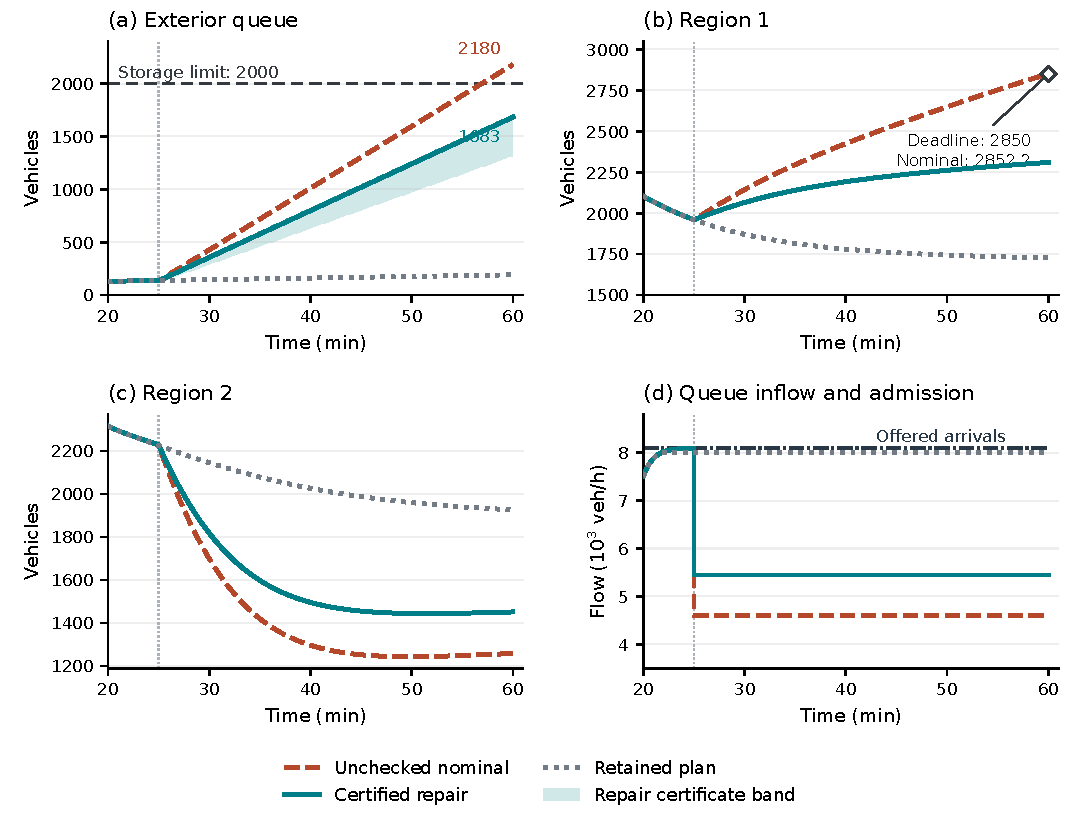
\includegraphics[width=\textwidth]{figures/supervisory_combined.pdf}
\caption{Matched queue--deadline conflict case: (a) exterior queue $z$,
(b) Region~1 accumulation $n_1$, (c) Region~2 accumulation $n_2$, and
(d) exterior arrivals $\Lambda$ and admission $a$, in thousands
of vehicles per hour. The three plans use identical initial states and
arrivals, and the vertical dotted line marks the control-input change at
minute 25. The horizontal line in (a) is the 2000-vehicle storage limit.
The shaded band bounds the repaired queue continuously on each
15-second proof interval for all one-vehicle initial half-widths and
measurable arrival errors bounded by 300~veh/h. Its upper bound
reaches 1682.7 vehicles. The marker in (b) is the 2850-vehicle requirement
at minute 60, where unchecked nominal execution ends at 2852.2 vehicles.
The 10,000-vehicle regional limits lie above the plotted ranges.
The repair and retained-plan certificates cover the full stated
uncertainty family through minute 60.}
\label{fig:supervisory-counts}
\label{fig:supervisory-flows}
\label{fig:certified-queue-bound}
\end{figure}

Figure~\ref{fig:supervisory-flows}(d) explains the queue response through
the arrival and admission rates. At minute 25, the nominal plan reduces admission to
approximately 4594~veh/h, so arrivals exceed entry to Region~2 and the
exterior queue grows. Repair raises admission to approximately
5447~veh/h and increases the Region-1-to-Region-2 perimeter control input from
0.397 to 0.548. These changes reduce exterior waiting and the number of
vehicles remaining in Region~1, while allowing a higher Region-2
accumulation than the nominal proposal. The queue continues to grow under
repair, but stays within storage through the certified minute-60 expiry.
The example illustrates the finite-plan guarantees of
Proposition~\ref{prop:structure-plan} and Lemma~\ref{thm:repair-grid}.



Table~\ref{tab:benchmark-conflict} quantifies this tradeoff and includes
the other planning options on the same realization. Retention gives the
lowest TTS, while repair lowers the Region-2-weighted cost relative to
retention. The physical control-barrier-function quadratic program
(CBF-QP) protects storage but misses the deadline. Full-scenario MPC
satisfies both constraints on this realization, although the certification check
for the full uncertainty family is inconclusive. Thus the table distinguishes the
observed traffic performance from the guarantee available for execution.
For the same realization, completed trips are 15,924 for nominal MPC,
16,770 for repair, and 18,365 for retention, rounded to whole vehicles.
These counts agree with the total-accumulation balance in
\eqref{eq:new-conservation} and help explain the lower TTS under retention.
The plotted trajectories use the stored control inputs and were checked by
independent adaptive integration against the original simulations and the
regional and queue conservation balances.

\begin{table}[!htbp]
\centering\footnotesize
\setlength{\belowcaptionskip}{6pt}
\caption{Matched adverse realization, minutes 20--60. TTS is total
time spent in the regions and exterior queue. $J_D$ weights Region~2 by
$p=4$. Both use veh-h. Costs and counts are rounded to whole
units. Peak queue is the maximum exterior count $z$. $n_1(E)$ is the
Region-1 count at deadline $E=60$ minutes. Their limits are 2000 and 2850
vehicles. P/S lists physical/service outcomes: P=pass, F=fail. Cert.
reports full-family certification: Yes=certified, No=not certified,
dash=not assessed by that certification procedure.
MPC means model predictive control, and CBF means control barrier function.
Retained continuation follows the previous certified plan. Nominal-plan
and Full-scenario repair interpolate their MPC proposals toward it.}
\label{tab:benchmark-conflict}
\setlength{\tabcolsep}{3pt}
\begin{tabular}{@{}lrrrrcc@{}}
\toprule
Policy & TTS & $J_D$ & Peak queue & $n_1(E)$ & P/S & Cert.\\
\midrule
Nominal MPC & 3300 & 6328 & 2180 & 2852 & F/F & No\\
Physical CBF & 3295 & 6376 & 1844 & 2917 & P/F & ---\\
Retained continuation & 2695 & 6814 & 194 & 1727 & P/P & Yes\\
Nominal-plan repair & 3097 & 6427 & 1683 & 2310 & P/P & Yes\\
Full-scenario MPC & 3267 & 6357 & 1999 & 2848 & P/P & No\\
Full-scenario repair & 3075 & 6453 & 1547 & 2314 & P/P & Yes\\
\bottomrule
\end{tabular}
\end{table}

The certificate band in Figure~\ref{fig:certified-queue-bound}(a)
leaves at least 317.3 vehicles of storage throughout the repair.
The \reproductiondetails{flow and enclosure records} also provide the
regional inflow/outflow plots and ten queue simulations against this band.



\subsection{Effects of uncertainty and traffic structure}
\label{sec:structure-results}
\label{sec:structure-online}
\label{sec:uncertainty-results}

We next examine how the traffic-specific bounds in
Section~\ref{sec:structure-certificate} affect certification as uncertainty
and service requirements vary.

\paragraph{Tighter bounds for a fixed plan}
The largest tested certifiable regional half-width is 50 vehicles with
signed propagation, compared with 10 vehicles for the interval methods,
at a 60~veh/h arrival-error bound. To separate the coordinate effect
from the propagation method, Table~\ref{tab:coordinate-comparison} compares
five representations for the same fixed two-block MPC plan, forecast,
initial state, and 15-second proof partition. Destination-class coordinates
give a 2075-vehicle deadline bound at $d=1$. Including the queue shares
reduces it to 1780 vehicles. Both representations pass through $d=10$ on
the tested grid, while checks using raw accumulation boxes remain inconclusive throughout
that grid.

\begin{table}[!htbp]
\centering\small
\setlength{\belowcaptionskip}{6pt}
\caption{Matched coordinate and enclosure comparison for one fixed MPC
plan over minutes 0--60. The arrival-error bound is 60~veh/h, the
deadline limit is 2850 vehicles, and the proof interval is 15 seconds.
The initial bound is
$d_x=(d,d,d,d,d,d,\min(d,10))^\top$ vehicles. All five methods test
$d\in\{1,5,10,25,50,100\}$. Deadline bounds are rounded upward to whole
vehicles. The largest passing $d$ is a tested grid value. None means no
complete certificate passes on this grid. The final column reports the
deadline bound at that method's largest passing $d$.}
\label{tab:coordinate-comparison}
\setlength{\tabcolsep}{4pt}
\begin{tabular}{@{}lrrr@{}}
\toprule
Representation & \shortstack{Bound at\\$d=1$} & \shortstack{Largest\\passing $d$} & \shortstack{Bound at\\largest $d$}\\
\midrule
Raw accumulations & --- & None & ---\\
Destination classes & 2075 & 10 & 2388\\
Conservation coordinates & 1780 & 10 & 1845\\
Positivity/queue & 1729 & 10 & 1777\\
Signed generators & 1722 & 50 & 1853\\
\bottomrule
\end{tabular}
\end{table}

The queue-capped uncertainty in Table~\ref{tab:coordinate-comparison}
differs from the equal seven-state half-widths used for minute-20
replacement. In particular, the 50-vehicle result retains a 10-vehicle
queue half-width. These are sensitivity settings whose field accuracy
requires calibration. At a larger 300~veh/h arrival-error bound and $d=1$,
positivity/queue propagation gives a tighter deadline bound than signed
propagation (2009 versus 2256 vehicles). At $d=25$, only the signed
method passes, with a 2504-vehicle bound. The refinements therefore give
complementary checks, and acceptance requires every constraint to pass.

In a separate service-margin study with a 1700-vehicle limit,
$d_x=\mathbf1_7$ vehicles, and a 60~veh/h arrival-error bound, signed
propagation certifies a nominal target of 1625 vehicles. The interval
methods first pass at 1600 on the tested target menu. This reduces the
margin from 100 to 75 vehicles and nominal TTS by 0.90\% (41 veh-h).
The complete uncertainty table, target menu, and feedback comparison
are in the \reproductiondetails{structure and service-margin records}.
The separate feedback comparison assumes exact state feedback.

\paragraph{Coverage across service and uncertainty requirements}
The broader regional-priority comparison returns to the common minute-20 state and
the 30\% one-hour event. Its 72 development contracts cross initial-state
half-widths $d\in\{1,10,25,50\}$ vehicles, arrival-error bounds
$\bar w\in\{60,150,300\}$ veh/h, deadline limits
$\eta\in\{2750,2850,2950\}$ vehicles, and Region-2 weights $p\in\{2,4\}$.
Eight held-out contracts use $d\in\{5,20\}$,
$\bar w\in\{100,225\}$, $\eta\in\{2800,2900\}$, and $p=3$.
Each two-block plan has 640 matched simulations. Full-scenario MPC constrains
these scenarios and the center forecast with one-vehicle prediction
clearance.

\begin{table}[!htbp]
\centering\small
\setlength{\belowcaptionskip}{6pt}
\caption{Regional-priority task with a service deadline: 72 development and eight held-out
contracts over minutes 20--60. Entries count passing contracts out of 80.
Simulation passes satisfy physical and service limits in all 640 simulations
(128 initial-state corners times five arrival-error profiles).
Certified passes establish continuous physical limits and the minute-60 service
bound for every allowed initial state and arrival error. MPC means model predictive control.
Nominal MPC plans from the state-set center with zero arrival error.
Five-scenario MPC adds the all-low/all-high states with both constant
arrival-error extremes. Full-scenario MPC uses all 640 combinations plus the
center forecast. All minimize center-forecast priority cost. Checked-repair
entries count all certified outputs: unchanged proposals and checked
interpolations toward a backup. New-backup construction (reserve refresh) supplies a newly certified
backup for nominal-plan repair when the previous continuation does not
pass the check for the current contract.}
\label{tab:benchmark-deadlines}
\begin{tabular}{@{}lrr@{}}
\toprule
Planning/execution option & Simulation passes & Certified passes\\
\midrule
Nominal MPC & 36/80 & 36/80\\
Five-scenario MPC & 40/80 & 40/80\\
Full-scenario MPC & 80/80 & 44/80\\
Nominal MPC with checked repair & 74/80 & 74/80\\
Full-scenario MPC with checked repair & 74/80 & 74/80\\
Repair with a newly certified backup & 80/80 & 80/80\\
\bottomrule
\end{tabular}
\end{table}

Table~\ref{tab:benchmark-deadlines} shows that full-scenario MPC passes
all tested simulations in every contract, while certification over the full
uncertainty family succeeds in 44/80. Checking the existing continuation against the current
contract establishes a certified backup in 68/80, and ordered repair
produces certified plans in 74/80. Newly constructed backups pass
certification in all twelve contracts where the previous continuation
does not pass, enabling repair in the remaining six. This illustrates
the same-contract backup requirement in Lemma~\ref{thm:repair-grid}.
Separately, the physical CBF-QP satisfies physical constraints in all
80 adverse runs and the deadline in 44, using one adverse realization per
contract. Its instantaneous physical barriers and the scheduled service
requirement therefore lead to different outcomes.

Across the 80 contracts, nominal MPC violates queue storage in 44
contracts and the service deadline in 36. Taking the largest observed
excess within each affected contract, queue overflow ranges from 36.0 to
242.7 vehicles, with median 90.3. Deadline excess ranges from 1.3 to
65.4 vehicles, with median 19.4. These are simulation-based violation sizes,
reported separately from inconclusive certification outcomes.

To quantify the traffic cost of repair, compare nominal, retained, and
repaired plans $P^0,P^B,P^R$ on a common realization $\omega$. The priority
improvement $\Delta J_\omega$, change in queue-inclusive delay
$\Delta D_\omega$, and recovered requested benefit $B_\omega$ are
\begin{equation}
\begin{aligned}
\Delta J_\omega&=100\frac{J_D(P^B;\omega)-J_D(P^R;\omega)}{J_D(P^B;\omega)},\\
\Delta D_\omega&=100\frac{J_Q(P^R;\omega)-J_Q(P^B;\omega)}{J_Q(P^B;\omega)},\\
B_\omega&=\frac{J_D(P^B;\omega)-J_D(P^R;\omega)}{J_D(P^B;\omega)-J_D(P^0;\omega)}.
\end{aligned}
\label{eq:benchmark-repair-metrics}
\end{equation}
Positive $\Delta J_\omega$ means that repair improves the priority
objective relative to retention, while positive $\Delta D_\omega$ means
that it increases TTS. These changes and $100B_\omega$ are percentages.
Across 24,320 matched realizations from the 38 contracts repaired using
the original continuation, every denominator in $B_\omega$ is positive.
Median priority improvement relative to retention is 5.7\%, median TTS
increase is 16.1\%, and median recovered requested benefit is 91.7\%.
Repair thus recovers much of the requested regional preference with a
measured increase in TTS. These realized costs complement the analytical
bound in Proposition~\ref{prop:repair-cost}, which requires its stated
common-domain and regularity assumptions.

\subsection{Successive requests and computation delays}
\label{sec:sequential-handover-results}

The preceding studies evaluate a decision from a specified initial set.
During repeated operation, each new request instead inherits the traffic
state produced by earlier decisions. We first examine replacements at
fixed activation times, then allow time for planning and certification.
The service deadline remains at minute 60 throughout both studies.

\paragraph{Successive plan requests}
A certified regional-priority repair with Region-2 weight $p=4$ starts at minute 20.
At minute 25, a request proposes the remaining $p=2$ full-scenario plan,
and at minute 30 another request proposes the remaining $p=4$ nominal
plan. These are stored planner outputs, used to isolate the supervisory
decision from language interpretation. Physical limits and uncertainty
bounds remain fixed. Each replacement is checked from a box containing
the states reachable under the active plan. Rejection preserves that
plan's original schedule, stored certificate, and expiry, as required by
Theorem~\ref{thm:new-plan-closure}.

\begin{table}[!htbp]
\centering\small
\setlength{\belowcaptionskip}{6pt}
\caption{Successive requests in the regional-priority task. The 25/30 column gives the
minute-25 and minute-30 decisions: A activates the replacement and R
retains the current plan. Feasible simulations satisfy physical limits and
the minute-60 service requirement, out of 640 matched realizations.
TTS includes exterior waiting over minutes 20--60, in veh-h. Retain keeps
the initial certified plan, Unchecked executes both requested replacements,
and Supervised executes only certified replacements. Medians include all
640 simulations. The first three cases were preselected; the tight-deadline
case is the first overflow found in the complete matched-pair scan.}
\label{tab:sequential-handover}
\setlength{\tabcolsep}{3pt}
\begin{tabular}{@{}>{\raggedright\arraybackslash}p{0.21\linewidth}cccccc@{}}
\toprule
Case & 25/30 & \multicolumn{2}{c}{Feasible simulations} & \multicolumn{3}{c}{Median TTS (veh-h)}\\
 & & Unchecked & Supervised & Retain & Unchecked & Supervised\\
\midrule
Low arrival error & A/A & 640/640 & 640/640 & 3196 & 3081 & 3081\\
Queue--deadline conflict & A/R & 640/640 & 640/640 & 3037 & 3081 & 2717\\
Wide initial uncertainty & R/R & 640/640 & 640/640 & 3169 & 3094 & 3169\\
Tight deadline & A/R & 512/640 & 640/640 & 2963 & 3070 & 2719\\
\bottomrule
\end{tabular}
\end{table}

Table~\ref{tab:sequential-handover} covers acceptance of both requests,
acceptance followed by retention, and retention at both decisions.
For the low-arrival-error, queue--deadline conflict, wide-initial-uncertainty,
and tight-deadline cases, respectively, the triples
$(d,\bar w,\eta)$ are $(1,60,2850)$, $(1,300,2850)$,
$(50,60,2950)$, and $(1,300,2750)$, respectively, in vehicles, veh/h,
and vehicles. In the queue--deadline conflict case, the service check for
the second request is inconclusive even though its sampled unchecked schedule satisfies the
constraints. In the wide-initial-uncertainty case, the propagated boxes include inadmissible states,
without establishing that an actual trajectory reaches them. These cases
show why an inconclusive certification check must be distinguished from a
demonstrated violation.

The development scan contains 36 matched weight pairs, of which 30 have
the certified source plans needed for the sequence. Unchecked switching
overfills storage in three of these 30 cases, all subsequently tested by
the sequential certification procedure. In the tight-deadline case in Table~\ref{tab:sequential-handover},
the minute-25 replacement passes,
but the minute-30 request fails the queue check. Executing both requests
unchecked reaches 2005.59 vehicles against the 2000-vehicle limit,
confirmed by independent adaptive integration. Retaining the accepted
plan gives 640/640 physically and service-feasible simulations. Its median
TTS is 8.2\% below retaining the initial plan, while its median
changing-priority cost is 5.2\% above unchecked switching. The three violating pairs have maximum queue excesses of 5.59, 9.62,
and 17.60 vehicles, respectively, against the 2000-vehicle capacity.
The full scan and the other overflow cases are in the
\reproductiondetails{successive-request records}.



\paragraph{Planning and checking before activation}
\label{sec:delayed-handover-results}
The delay study tests Proposition~\ref{prop:planned-handover} using
seventeen contracts with one-, two-, and five-minute preparation slots,
giving 51 cases. The current plan executes while its reachable set is
propagated to the scheduled activation time. A replacement is checked
from that future state set through the unchanged deadline.

\begin{table}[!htbp]
\centering\small
\setlength{\belowcaptionskip}{6pt}
\caption{Replacements with delayed activation. The handover slot is the
preparation time after minute 20. Replacements and retentions count timely
certified activations and continued execution of the prior plan,
respectively, out of seventeen contracts per slot. Feasible trajectories
satisfy physical limits and the minute-60 service requirement. Each row
contains $17\times640=10{,}880$ matched initial-state/arrival simulations.}
\label{tab:delayed-handover}
\setlength{\tabcolsep}{4pt}
\begin{tabular}{@{}lrrr@{}}
\toprule
Handover slot & Replacements & Retentions & Feasible trajectories\\
\midrule
1 minute & 8/17 & 9/17 & 10,880/10,880\\
2 minutes & 11/17 & 6/17 & 10,880/10,880\\
5 minutes & 11/17 & 6/17 & 10,880/10,880\\
\bottomrule
\end{tabular}
\end{table}

Table~\ref{tab:delayed-handover} reports 30 timely replacements and
21 retentions, with all 32,640 simulations satisfying the physical and service
constraints. Three one-minute results arrive too late. Longer preparation
provides more computation time, but it also changes the reachable state
set and shortens the remaining service horizon. This explains why the
number of accepted replacements need not increase with the slot length.
In addition, replacing a reachable set by separate bounds on each state component can prevent
certification of a replacement even though the current plan retains its
original certificate.

\paragraph{Computation time for the seven-state model}
Three repeated measurements of the queue--deadline conflict case on an
Intel Core Ultra 7 255H computer with Windows 11 and Python 3.12.10 give
a median nominal-plan check of 8.1~s (range 8.1--8.3~s).
Checking the proposal and the five repair candidates through
$\lambda_{\rm rep}=0.25$ takes a median 52.7~s (range 51.6--52.9~s).
Rechecking the backup as well raises this to 63.4~s (range 62.2--63.7~s).
Each candidate starts a fresh verifier. These measurements exclude
planning, trajectory simulation, plotting, and module imports. Across the
38 original repairs in the full contract scan, the recorded time spent
checking additional grid candidates ranges from 8.3 to 175.9~s, with
median 17.6~s. That scan includes different numbers of tested candidates
and the original evaluation workload. The delayed-handover study above
uses its own recorded total preparation times, including propagation,
planning, and checking. Observed runtimes inform preparation windows,
while acceptance still requires completion before the chosen activation.

\subsection{Agent interpretation and certified execution}
\label{sec:task-state-live}
\label{sec:queue-live-pilot}
\label{sec:primary-memory-pressure}

The agent study evaluates whether the AI agent selects the intended
objective and whether the executed plan satisfies the physical and service
requirements. It compares the history-only and task-record interfaces
defined in Section~\ref{sec:agent-requests}.

The recorded model is \texttt{gpt-5.4-mini-2026-03-17}, with reasoning
disabled and strict function schemas specifying the required fields and
allowed values in tool requests. A 96-call interpretation pilot crosses
three tool-availability situations, four operator histories, clean or
corrupted memory, two interfaces, and two repetitions. It routes
precomputed plans. The corrupted memory requests a changed priority,
increased storage limit, or unchecked execution. Objective correctness is
measured against the active operator instruction, and tool correctness
against the stored certified-tool selection rule.

\begin{table}[!htbp]
\centering\small
\setlength{\belowcaptionskip}{6pt}
\caption{Agent interpretation and actual planning. Top: the pilot uses
24 calls per interface/memory pair. History only supplies reported traffic information
and interaction memory. Task record also supplies the active priority,
expiry, and interruption status. Clean memory is unaltered, while corrupted
memory contains misleading instructions. Objective correct means agreement
with the active operator priority, and tool correct means agreement with
the saved certified-tool selection rule. Bottom: actual planning uses
four traces per interface under corrupted memory. Objective correct
assesses the initial requests. Repairs executed counts traces activating
a certified grid repair. Feasible trajectories satisfy the physical and
service requirements in $4\times640=2560$ simulations per interface.}
\label{tab:benchmark-api-pilot}
\label{tab:benchmark-api-execution}
\setlength{\tabcolsep}{4pt}
\begin{tabular}{@{}llrr@{}}
\toprule
Pilot interface & Memory & Objective correct & Tool correct\\
\midrule
History only & Clean & 19/24 & 22/24\\
History only & Corrupted & 15/24 & 24/24\\
Task record & Clean & 24/24 & 24/24\\
Task record & Corrupted & 24/24 & 24/24\\
\midrule
Actual planning & Objective correct & Repairs executed & Feasible trajectories\\
\midrule
History only & 1/4 & 1/4 & 2560/2560\\
Task record & 4/4 & 4/4 & 2560/2560\\
\bottomrule
\end{tabular}
\end{table}

Table~\ref{tab:benchmark-api-pilot} shows that the task record improves
objective selection in these paired examples: it gives 24/24 correct
objectives with both clean and corrupted memory, compared with 19/24 and
15/24 for history alone. The two clean-memory tool errors select
retention when the stored rule prefers a certified repair. Both actions
preserve certified execution. The higher tool score under corrupted
memory coexists with poorer objective selection (15/24), illustrating
why the two scores are reported separately.

A separate actual-planning study uses eight
traces, each a recorded sequence of requests, tool responses, and execution
decisions. The traces pair four histories across the two interfaces under
corrupted memory and use the agent's selected objective in a fresh MPC
solve. The interface forwards the generated plan directly to the
supervisor. Following rejection, the agent receives feedback and can request
repair or retention. Repair is attempted only when the agent requests it,
and every repair is checked before execution. The traces test objective
selection and repair responses from the supplied histories, rather than
every operation in Table~\ref{tab:task-operations}.
They contain thirteen live calls and 640 simulations per executed schedule.

In three history-only traces, the accepted MPC plan satisfies the physical
and service requirements but pursues the wrong regional objective.
Only one history-only trace executes a checked repair, compared with
all four task-record traces. All 2560 simulations for each interface satisfy
the physical and service limits. These outcomes demonstrate the distinct
roles of the task record and the supervisor: the record supports correct
objective selection, while certification enforces the independently
supplied constraints on each accepted plan, as formalized in
Corollary~\ref{cor:agent-independent-execution}. The results describe a small
study with one recorded model version, evaluated through the accepted
plans' finite execution intervals. Essential histories and scoring rules
are in \appref{sec:supp-execution}, with prompts, replies, and simulation
instructions in the \reproductiondetails{agent experiment records}.

\subsection{Extension to several entry queues}
\label{sec:network-transfer-results}

To examine the network construction in
Proposition~\ref{prop:network-localization}, we also certify fixed plans
on connected two- and three-region rings with six and twelve states.
Each region has an exterior entry queue. This study uses its own fixed
routing and allocation assumptions, specified in
\appref{app:network-transfer}.

At regional half-width $d=25$ vehicles, the combined accumulations certify
the two-region plan with a 300~veh/h arrival-error bound per queue and the
three-region plan with a 60~veh/h bound. Their largest regional deadline
bounds are 1552 and 2060 vehicles against a 2700-vehicle limit.
Class coordinates alone leave both certification checks inconclusive.
Successful twelve-state proofs take 5.20--5.28 seconds for 120 intervals.
The full sixteen-attempt sweep and runtime records are in the
\reproductiondetails{connected-network study}.



\section{Operational Insights and Implementation}
\label{sec:new-discussion}
\label{sec:information-model-scope}

Admission and interregional transfers must
be coordinated because reducing entry to a region can increase its
exterior queue. Traffic-specific bounds allow more plans to be accepted
under the same information and service requirements, while wider
uncertainty may require a newly certified backup.

The studies use a literature MFD, synthetic internal demands, and known
event means. Certificates cover the stated initial-state uncertainty and
exterior-arrival errors, with MFD outflow, routing, internal demand, release rate,
and entrance capacity fixed. Since regional totals leave destination mixtures
undetermined, deployment requires a joint set containing the actual
class accumulations and queues, including measurement bias and timing
errors. Destination decomposition is also treated as uncertain in robust
perimeter control \cite{haddad2015robust}. The one-vehicle cases here
describe tightly known initial conditions, and the wider sweeps assess
sensitivity under their stated queue bounds. Field use requires calibrated
state and arrival-error sets, together with validated bounds for any
additional model uncertainty. Section~\ref{sec:network-extension} states
the fixed-allocation assumptions. Feedback execution using estimates
also requires bounds on how measurement and timing errors affect the
applied controls throughout execution.

Deployment requires a certified initial plan, certificates matching current
model and task versions, and enough time for propagation, planning,
checking, and actuation before expiry, accounting for hardware and load.
Continuation beyond expiry also requires the invariant policy, terminal-set
inclusion, and service coverage in \appref{sec:terminal-backup},
with sustained arrivals compatible with storage and discharge.

\section{Conclusions}
\label{sec:new-conclusion}

This paper develops a dual-agent framework in which an AI agent proposes
urban perimeter-control plans and a rule-based supervisory agent checks
them before execution. Under the stated traffic model and execution
assumptions, the framework verifies physical constraints and service
deadlines for every activation state and arrival allowed by the supplied
bounds. Vehicle conservation and the links between boundary queues and
regional traffic tighten bounds on future states. Plans that pass
certification can be executed unchanged, and checked repair searches for
certified alternatives. Rejected or late replacements leave the previously
accepted plan in use for the period covered by its certificate. When the
required terminal conditions are also certified, these guarantees can
continue beyond the planned control period. Numerical studies show reduced
conservatism and recovery of plans that meet the requirements through
repair. Further experiments examine
successive requests, computation delays, and errors in the information
given to the agent, with certified execution maintained in the tested
cases. Connected-network examples demonstrate the extension to several
entry queues.

Future work will focus on estimating vehicle counts by region and
destination from traffic measurements, calibrating the associated
uncertainty bounds, and incorporating estimation errors into feedback
certification. Another direction is to establish uncertainty bounds
that capture differences between the traffic model and observed network
behavior. We will also study when new plans should take effect, accounting
for sensing, computation, and actuation time, traffic uncertainty, and
remaining service deadlines. These developments will support evaluation of
the framework in operational traffic networks.

\section*{CRediT authorship contribution statement}
\textbf{Ali Eslami:} Conceptualization, Methodology, Software, Validation,
Formal analysis, Investigation, Data curation, Visualization,
Writing and editing.
\textbf{Jiangbo Yu:} Supervision, Review and editing.

\section*{Declaration of competing interests}
The authors declare that they have no known competing financial interests or
personal relationships that could have appeared to influence the work
reported in this paper.

\section*{Data and code availability}
Reproducibility materials include the traffic models, planning and
certification implementations, experiment protocols, stored agent requests
and responses, proof records, and simulation outputs described in the
experimental settings in \appref{app:experimental-settings}. The materials are maintained at
\url{https://github.com/AlienEslami/agentic-perimeter-runtime-certification}.


\appendix
% Use appendix letters for equations while retaining full appendix section titles.
\renewcommand{\theequation}{\Alph{section}.\arabic{equation}}
\numberwithin{table}{section}
\renewcommand{\thetable}{\Alph{section}.\arabic{table}}
\Needspace{0.78\textheight}
\section{Notation}
\label{app:notation}

\begingroup
\fontsize{9}{10}\selectfont
\renewcommand{\arraystretch}{0.98}
\setlength{\LTcapwidth}{\textwidth}
\begin{longtable}{@{}p{0.20\linewidth}>{\raggedright\arraybackslash}p{\dimexpr0.80\linewidth-2\tabcolsep\relax}@{}}
\caption{Notation used throughout the paper. Traffic accumulations and state bounds are in vehicles,
flow rates are in veh/h, and time is in hours unless stated otherwise.}
\label{tab:nomenclature}\\
\toprule
Symbol & Meaning\\
\midrule
\endfirsthead
\multicolumn{2}{@{}l@{}}{Table~\thetable\ (continued)}\\
\toprule
Symbol & Meaning\\
\midrule
\endhead
\midrule
\endfoot
\bottomrule
\endlastfoot
$n_i$, $n_{ij}$ & Regional accumulation; vehicles in region $i$ destined for $j$\\
$z$, $x$, $M$ & Exterior queue; traffic state; total vehicle accumulation\\
$\widehat x_{t_0}$, $\mathcal I_{t_0}$ & Supplied state estimate and containing state set at plan activation\\
$u_{ij}$, $a$ & Perimeter control input; realized exterior admission flow\\
$G_i$, $m_{ij}$ & Regional MFD outflow; potential destination-class flow\\
$v(n)$ & Per-vehicle outflow rate $G(n)/n$ (h$^{-1}$)\\
$\pi$, $\tau_q$, $\kappa_{02}$ & Region-1 entry fraction; queue-release time; admission capacity\\
$n_i^{\max}$, $z^{\max}$ & Regional operational accumulation limit; exterior storage capacity\\
$\delta_1^u$, $\delta_2^u$ & Allowed differences between paired perimeter control inputs\\
$\Lambda$, $\widehat\Lambda$, $w$ & Exterior arrival rate, forecast, and forecast error\\
$d^{\rm int}_{ij}$ & Internal demand in region $i$ for destination $j$ (veh/h)\\
$d_x$, $d_x(t_i)$, $d$ & Initial state-error bounds, bounds at $t_i$, and scalar sweep parameter\\
$\bar w$ & Arrival-forecast error bound (veh/h)\\
$\mathcal S_t$, $\mathcal S_t^{\rm rep}$ & Full decision record and its repair fields\\
$\mathcal H_t$, $\mathsf v_t$ & Current certificate; model, forecast and constraint versions\\
$\mathcal O_t$, $\mathcal W_t$ & Pending service requirements; allowed arrival-error family\\
$P$, $P_i^0$, $P_i^{\rm cand}$ & Generic plan, original proposal, and candidate (original or repaired)\\
$P_t^{\rm cur}$, $E_{\rm cur}$ & Current executing plan and its original expiry\\
$P^B$, $E_B$, $\mu_{\rm term}$ & Repair backup, its expiry, and terminal policy beyond expiry\\
$t_i^{\rm req}$, $t_i$, $t_{\rm ready}$ & Request, decision/activation, and certificate-completion times\\
$T^{\rm prio}$, $E$ & Priority expiry; plan expiry\\
$\mathsf{Comp}$, $q_i^A$ & Request compiler; validated planning request ($\bot$ if invalid)\\
$P_a$, $c$ & Destination-allocation matrix; network destination-class vector\\
$n_{\rm cls}$, $n_q$ & Numbers of network destination classes and entry queues\\
$\gamma_i^{\rm rel}$, $u_i^{\rm in}$ & Network queue-release rate (h$^{-1}$) and entrance input\\
$\eta$ & Regional-priority task's Region-1 accumulation limit (vehicles)\\
$T_r$, $g_r$, $\eta_r$ & Service deadline, constraint coefficients and limit\\
$\theta_i$, $\lambda_{\rm rep}$ & Agent task record; predictive-repair interpolation weight\\
$K_b$, $N_b$, $\mathcal K$ & Feedback gain; control-block count; terminal invariant set\\
$\beta_j^{\rm phys}$, $b_a$ & Physical constraint limit; vehicle-admission incidence vector\\
$y$, $L$ & Conservation-coordinate state and its invertible transform\\
$r_l$, $R_l$ & Initial error bounds and trial error bounds on interval $l$\\
$r^{\rm gen}$, $r^\zeta$ & Continuous bounds on signed-generator and remainder contributions\\
$a_{il}$, $b_{ijl}$ & Local diagonal and off-diagonal Jacobian bounds\\
$\xi$, $\Gamma_l$, $\zeta_l$ & Shared initial uncertainty, its coefficient matrix and error remainder\\
$z_e$ & Prediction-error coordinate used only in the enclosure proof\\
$J_Q$, $J_D$ & Queue-inclusive and weighted-priority objectives\\
$p$, $\mathbf p_l$ & Regional-priority weight; state predictor\\
$\mathcal C$, $\mathcal F_{\mathcal C}$, $\widehat{\mathcal F}_{\mathcal C}$ & Planning contract; robustly feasible and certified plan sets\\
$\overline M$, $\Psi$ & Metzler comparison matrix; integral of its exponential\\
$N_{\rm T}$, $v_{\rm term}^{\max}$ & Matrix-series order; terminal Lyapunov level\\
$B_\omega$ & Fraction of requested priority benefit recovered by repair\\
$\mathrm{TTS}$ & Total time spent, including exterior waiting; vehicle-hours (veh-h)\\
\end{longtable}
\endgroup

\section{Essential Experimental Settings}
\label{app:experimental-settings}
\label{app:reusable-benchmark}
\label{sec:supp-queue-settings}
\label{app:benchmark-details}

\paragraph{Implementation coordinates}
The stored numerical implementation represents 100 vehicles as one unit.
For implementation state $\widetilde x=x/100$, physical-unit and stored
quantities satisfy
\[
\widetilde f(\widetilde x,u,t)=f(100\widetilde x,u,t)/100,\qquad
\widetilde w=w/100,\qquad
\widetilde G(\widetilde n)=G(100\widetilde n)/100.
\]
Control inputs and time are unchanged. A stored feedback law
$u=\widetilde k_b+\widetilde K_b\widetilde x$ corresponds to
$k_b=\widetilde k_b$ and $K_b=\widetilde K_b/100$ in this paper.
Stored predictors, state radii, signed generators, and additive error
bounds are multiplied by 100 to obtain their physical-unit values.
The transform $L$ is unchanged, and
$D_{\widetilde x}\widetilde f=D_x f$ at corresponding states and controls.
For a physical constraint $Hx+Ju\le\beta$, the equivalent stored form is
$100H\widetilde x+Ju\le\beta$.
A service limit $g^\top x\le\eta$ becomes
$100g^\top\widetilde x\le\eta$.
These conversions preserve the represented trajectories, control inputs,
and constraint satisfaction. Reported costs and vehicle counts already
use physical units.

\paragraph{Primary state and plans}
The network-efficiency and regional-priority tasks start at minute 20 with the state center, in the order of
\eqref{eq:new-state}, in vehicles,
\[
\begin{aligned}
\widehat x_{20}=(&2102.0544601495207,2315.6747836310867,\\
&1420.9387548878382,1487.7124601919054,\\
&240.28346640030684,301.84193919155455,\\
&124.10781134202304).
\end{aligned}
\]
The original continuation uses $(1,1,0.667015677,1)$ in control-input order
$(u_{12},u_{21},u_{02},u_{20})$, in five- and
35-minute blocks ending at minute 60. The continuation is rechecked for
each contract. If a new backup is needed, construction tries network TTS
followed by moderate Region-2 priority and certifies the result before
repair. The ordered repair grid is given in Section~\ref{sec:experimental-setup}.
Plans are converted to control-input coefficients and checked against exact
actuator constraints. State/service proof intervals are 15 seconds.

\paragraph{Trajectory simulations and comparisons}
Simulations use the five arrival-error profiles in
Section~\ref{sec:experimental-setup}, paired with all 128 initial-box
corners for constant plans. The CLF comparison uses sixteen corners,
every eighth entry of the lexicographic $\{-1,+1\}^7$ list.
Simulations use fourth-order Runge--Kutta
(RK4) integration with ten-second steps, supplemented by independent
adaptive eighth-order Runge--Kutta (DOP853) integration and conservation
checks. CLF and CBF comparators use exact simulated states at ten-second
updates, with constant control inputs between updates.
The CLF extension combines regional-error correction with
linear-quadratic admission/exit feedback and reference totals
$(2700,3200)$ vehicles. Its full tuning is in the repository records. The physical CBF-QP minimizes deviation from
MPC subject to control-barrier-function inequalities for the physical constraints, with gain $6$ h$^{-1}$
and the worst queue-arrival error \cite{ames2017}. Its service deadline
is an evaluation criterion. Solver details and validation records are in
\reproductiondetails{the primary experiments}.

\paragraph{Future activation}
\label{supp:detail:sec:delayed-handover-results}
\label{app:sequential-handover}
The seventeen handover contracts comprise the eight extremes
$(d,\bar w,\eta,p)\in\{1,50\}\times\{60,300\}\times
\{2750,2950\}\times\{4\}$, primary $(1,300,2850,4)$ contract and eight
held-out contracts. The active plan supplies the activation box
$\mathcal I_{t_a}^+=\widehat x_{t_a}+[-d_x(t_a),d_x(t_a)]$, where
$(d_x(t_a))_i=\sum_j|(L^{-1})_{ij}|(r_{t_a})_j$, by outward conversion of its
endpoint bound that preserves shared uncertainty dependence. Timed preparation includes propagation,
optimization, checking and repair.

\paragraph{Connected rings}
\label{app:network-transfer}
The ring model has $R=2$ or $3$ regions, classes $c_{ij}$ and one
queue per region. Regional and perimeter-input indices start at zero. The regional
total is $N_i=\sum_jc_{ij}$. Local completion is $c_{ii}v(N_i)$, nonlocal
transfer is $u_i c_{ij}v(N_i)$, and admission is $a_i=\min\{60z_i,12{,}000u_i^{\rm in}\}$. Nonlocal
vehicles move one edge and retain their destination. Half the admitted
traffic is local, and the rest is equally divided among other destinations.
Initial regional/queue totals are 3000/200 vehicles, with half the regional
traffic local. Per region, internal demand is 6000 local and 500 nonlocal
veh/h. Exterior arrivals are 4000 veh/h. Queue 0 has a 30\%
increase from minute 15 to 45. Ring/entrance inputs start at 0.65/0.50.
After minute 30, ring inputs 0/1 become 0.80/0.55 and entrance input 0
becomes 0.60, with other inputs unchanged. The vector $d_x$ has class components $d/R$ and queue components
$\min(d,10)$ vehicles. The regional deadline is 2700 vehicles
at one hour. Physical capacities match the primary model. The plan is
fixed before certification. \reproductiondetails{The ring experiment}
gives the remaining uncertainty pairs, certification procedure settings and all sixteen
outcomes.

\paragraph{Agent histories and scoring}
\label{sec:supp-execution}
The four histories cover direct instruction, restoration after one or
nested interruptions, and interruption expiry at minute 20. The pilot's presaved cases are a queue-only MPC plan with a 20\%
arrival increase lasting 30 minutes, a repair case with
$(d,\bar w,\eta,p)=(1,60,2750,4)$, and the same repair
case with replacement tools unavailable. Actual planning uses the
queue--deadline conflict case in Section~\ref{sec:new-incident-protocol}.
Objectives set weights on $(n_1,n_2,z)$ to $(1,1,1)$, $(4,1,1)$ or
$(1,4,1)$ for network, Region~1 or Region~2. Pilot tool correctness uses the saved
certification procedure ordering: certified economic MPC, certified scenario MPC,
checked repair, then retention. Detailed histories, schemas and raw
calls are in \reproductiondetails{the agent protocol}.

\section{Verified Numerical Evaluation}
\label{app:verified-arithmetic}

Acceptance bounds round coefficients, ranges, and comparison functions
outward: lower bounds downward and upper bounds upward, preserving all
allowed values. Generated predictors and trial radii support acceptance
only after these inequalities pass. For $K_b=0$, control-input constraints
are constant. Their stored binary coefficients are exact binary rationals,
so residuals, including zero, are checked exactly. State and storage
constraints still require verified trajectory bounds. This admits control inputs
on closed input boundaries without enlarging the control box.

Numerical evaluation of the matrix functions also needs verified error
bounds. For $\alpha\ge\|A\|_\infty$, $\sigma=\alpha h$, and series order $N_{\rm T}$,
\begin{equation}
 \begin{aligned}
 \left\|e^{Ah}-\sum_{k=0}^{N_{\rm T}}\frac{A^kh^k}{k!}\right\|_\infty
       &\le e^\sigma\frac{\sigma^{N_{\rm T}+1}}{(N_{\rm T}+1)!},\\
 \left\|\int_0^h e^{As}\,ds-
          \sum_{k=0}^{N_{\rm T}}\frac{A^kh^{k+1}}{(k+1)!}\right\|_\infty
       &\le he^\sigma\frac{\sigma^{N_{\rm T}+1}}{(N_{\rm T}+2)!}.
 \end{aligned}
 \label{eq:structure-matrix-tails}
\end{equation}
The norm exponential series gives the first bound. Integration with
$e^{\alpha s}\le e^{\alpha h}$ gives the second. Signed row coefficients
are formed before interval-time evaluation. Outward rounding covers every
coefficient, tail, product, sum, and generator conversion used in the
preceding tests. Equivalent scalar evaluation shortcuts and regression
records are provided with the repository implementation.

\section{Task-Record Operations}
\label{app:task-operations}

The task record converts instructions into a current objective while
tracking interrupted priorities and their absolute expiries. The complete
update rules are given in Table~\ref{tab:task-operations}. They affect the
objective requested from the planning tool without modifying the service
requirements maintained by the supervisor.

\begin{table}[H]
\centering\small
\caption{Task-record operations. A duration $D$ is expressed here in
hours. Suspended priorities retain their original absolute expiries.
Before each operation, an expired active priority is replaced by the
most recently interrupted unexpired priority, if one exists. With no
active priority, the objective is network efficiency. \appref{sec:supp-execution} specifies the operations exercised in
the agent histories.}
\label{tab:task-operations}
\begin{tabularx}{\textwidth}{@{}l>{\raggedright\arraybackslash}X>{\raggedright\arraybackslash}X@{}}
\toprule
Operation & Effect on $\theta_i$ & Resulting objective\\
\midrule
Set & Clear interrupted priorities and assign a new priority with
$T^{\rm prio}=t_i^{\rm req}+D$. & Newly requested regional objective.\\
Interrupt & Save the active priority, if any, then assign a temporary
priority with expiry $t_i^{\rm req}+D$. & Temporary regional objective.\\
Continue & Keep the active record and its expiry. & Current objective.\\
Extend & Add $D$ to the active expiry. Reject if no active priority
remains. & Current regional objective.\\
Resume & Restore the latest unexpired interrupted priority. If none
survives, apply the rule below. & Restored regional objective or network
efficiency.\\
Cancel & Clear both the active and interrupted priorities. & Network
efficiency.\\
\bottomrule
\end{tabularx}
\par\smallskip\raggedright\footnotesize
For Resume, if no interrupted record exists and the active priority is
not temporary, that priority is preserved. Otherwise, if no interrupted
priority survives, the active priority is cleared. The accepted operation \texttt{network} has the same effect as Cancel.
An interruption is rejected when it would exceed the four-record stack
limit.
\end{table}

\section{Continuation Beyond Plan Expiry}
\label{sec:terminal-backup-main}
\label{sec:terminal-backup}

A finite-plan certificate covers execution through its expiry $E$, which
is preserved after rejection. Coverage beyond $E$ requires a replacement
activated by $E$ with a later certified expiry or a certified terminal policy activated at $E$. If neither is available, the finite-plan result
establishes feasibility only through $E$.

In this framework, indefinite continuation uses a nonempty certified set
$\mathcal K$ and an implementable feedback policy $\mu_{\rm term}$. For every
activation state in $\mathcal K$ and every allowed uncertainty realization,
the terminal-policy trajectory exists for all future time, stays in $\mathcal K$,
and satisfies the physical state and input constraints. Policy
initialization is part of the certificate. The state-feedback policy
$\mu_{\rm term}(x)$ below assumes access to the exact values of the state components
on which it depends. An implementation using estimates requires its
measurement errors to be covered by the terminal certificate.

The following Lyapunov sublevel-set test \cite{khalil2002nonlinear}
provides sufficient conditions for a terminal policy. Applying it to the
queue-augmented model requires a verified policy, invariant set, and
service coverage. The control-Lyapunov-function (CLF) comparison in
Section~\ref{sec:new-evidence} is evaluated over finite plans and has
no such terminal certificate.

\begin{proposition}
\label{prop:backup-lyapunov}
Suppose the implemented terminal policy has closed-loop dynamics
\[
\dot x=g_{\rm term}(x,w_{\rm term}),\qquad w_{\rm term}(t)\in\mathcal W_{\rm term},
\]
where $\mathcal W_{\rm term}$ is compact, $w_{\rm term}(\cdot)$ is measurable, and $g_{\rm term}$ is
continuous and locally Lipschitz in $x$, uniformly over
$w_{\rm term}\in\mathcal W_{\rm term}$, on an open domain $\Omega$. Let
$V_{\rm term}:\Omega\rightarrow\mathbb R_{\ge0}$ be continuously differentiable and define
\[
\mathcal K=\{x\in\Omega:V_{\rm term}(x)\le v_{\rm term}^{\max}\},
\]
where $\mathcal K$ is nonempty and compact. If, on a neighborhood of
$\mathcal K$,
\[
\nabla V_{\rm term}(x)^\top g_{\rm term}(x,w_{\rm term})
\le -\lambda_{\rm term} V_{\rm term}(x)+\bar d_{\rm term}
\]
for all $w_{\rm term}\in\mathcal W_{\rm term}$, with
$\lambda_{\rm term}>0$ and
$0\le\bar d_{\rm term}\le\lambda_{\rm term} v_{\rm term}^{\max}$, and if every state and input generated
on $\mathcal K$ satisfies the authorized physical constraints, then
$\mathcal K$ is robustly invariant under $\mu_{\rm term}$.
\end{proposition}

\begin{proof}
For a trajectory starting in $\mathcal K$ at $t_a$, the chain rule
and the assumed derivative bound give, almost everywhere in the stated
neighborhood,
$\frac{d}{dt}V_{\rm term}(x(t))\le-\lambda_{\rm term} V_{\rm term}(x(t))+\bar d_{\rm term}$.
An integrating factor yields
\[
 V_{\rm term}(x(t))\le e^{-\lambda_{\rm term}(t-t_a)}V_{\rm term}(x(t_a))+
 \frac{\bar d_{\rm term}}{\lambda_{\rm term}}\bigl(1-e^{-\lambda_{\rm term}(t-t_a)}\bigr)
 \le v_{\rm term}^{\max}.
\]
The right-hand side is a weighted average of two quantities bounded by
$v_{\rm term}^{\max}$. This comparison excludes departure from the sublevel set.
Compactness of $\mathcal K$ within the open domain, together with the
stated uniform local regularity, allows the solution to continue for
all future times. The physical constraints hold on $\mathcal K$ by
assumption, proving robust invariance under every allowed uncertainty.
\end{proof}

A plan activated at $t_i$ with expiry $E_i>t_i$ is terminally certified
when it passes the physical and service checks on $[t_i,E_i]$, covers
every service requirement pending at activation at a deadline in that interval,
and its entire terminal reachable set satisfies
\begin{equation}
\mathcal R_i(E_i)\subseteq\mathcal K.
\label{eq:backup-terminal-landing}
\end{equation}
Its certificate specifies an implementable transition to $\mu_{\rm term}$ at
$E_i$, including required initialization. For
Proposition~\ref{prop:backup-lyapunov}, a sufficient test is
\begin{equation}
\sup_{x\in\mathcal R_i(E_i)}V_{\rm term}(x)\le v_{\rm term}^{\max}.
\label{eq:backup-computable-landing}
\end{equation}
Write $\mathsf{Cert}^{\mathcal K}_t$ for the certification procedure augmented with
these terminal conditions. Thus
\begin{equation}
\mathsf{Cert}^{\mathcal K}_t(P\mid\mathcal S_t)=1
\ \Longrightarrow\ \mathsf{Cert}_t(P\mid\mathcal S_t)=1.
\label{eq:terminal-checker}
\end{equation}
Acceptance additionally verifies terminal inclusion
\eqref{eq:backup-terminal-landing}, coverage of every pending deadline,
and an implementable transition to $\mu_{\rm term}$. Here the terminal enclosure
$\mathcal R_P(E_P)$ covers every trajectory in $\mathcal X_P$.

The following theorem carries this terminal guarantee through successive
replacements and activates the terminal policy when the active plan expires.

\begin{theorem}
\label{thm:backup-recursive-availability}
Let $\mu_{\rm term}$ be a certified terminal policy on $\mathcal K$. Enumerate
actual plan activations as $t_0^{\rm act}=t_0<t_1^{\rm act}<\cdots$,
with plans $P_k$ and expiries $E_k$. Suppose
\[
\mathsf{Cert}^{\mathcal K}_{t_k^{\rm act}}
 (P_k\mid\mathcal S_{t_k^{\rm act}})=1,\qquad
x(t_k^{\rm act})\in\mathcal I_{t_k^{\rm act}},
\]
and suppose every activation preserves all pending service requirements.
Assume $\#\{k:t_k^{\rm act}\le T\}<\infty$ for every finite $T$, and
that execution and uncertainty satisfy the active certificate. Let $k(t)=\max\{k:t_k^{\rm act}\le t\}$, and suppose execution follows
\begin{equation}
u^{\rm exec}(t)=\begin{cases}
u_{P_{k(t)}}(t,x(t)),&t<E_{k(t)},\\
\mu_{\rm term}(x(t)),&t\ge E_{k(t)}.
\end{cases}
\label{eq:terminal-execution-policy}
\end{equation}
Suppose the certified policy initialization is applied at expiry, and
a new service requirement during terminal-policy operation is accepted
only through a covering terminally certified plan. Then the trajectory exists for every $t\ge t_0$, and
\begin{equation}
\begin{aligned}
H_jx(t)+J_ju^{\rm exec}(t)&\le\beta_j^{\rm phys},
 &&t\ge t_0,\\
g_r^\top x(T_r)&\le\eta_r,
 &&\text{accepted service requirements with }T_r\ge t_0.
\end{aligned}
\label{eq:terminal-global-guarantee}
\end{equation}
Rejection preserves the active plan and its terminal transition.
\end{theorem}

\begin{proof}
Each activated plan contains the actual activation state and is certified
for the allowed uncertainty. Theorem~\ref{thm:new-plan-closure} gives
its physical and service guarantees until replacement or expiry.
If the next plan starts at or before $E_k$, its matching certificate
continues that guarantee. Otherwise,
\[
 x(E_k)\in\mathcal R_{P_k}(E_k)\subseteq\mathcal K,
 \qquad x(t)\in\mathcal K\quad(E_k\le t<t_{k+1}^{\rm act}),
\]
because the certified initialization activates $\mu_{\rm term}$ at expiry.
Its invariant-set certificate covers that interval, indefinitely if
no further activation occurs. Rejection preserves this same terminal
transition. Only finitely many plans are activated in any finite
interval, so the certified plan and terminal-policy segments define
a solution for every $t\ge t_0$ and satisfy the physical constraints.

Every activated plan covers all pending service requirements
within its horizon, and replacements preserve that coverage. At a
deadline, the covering certificate gives $g_r^\top x(T_r)\le\eta_r$.
By expiry, all service deadlines assigned to that finite plan have been covered.
During terminal-policy operation, a new request is accepted only
through a covering terminally certified plan. Thus every accepted service
requirement is met, proving \eqref{eq:terminal-global-guarantee}.
\end{proof}

A service request made during terminal-policy operation is accepted
only after a new certificate covers that request and a terminal
continuation. A nonempty invariant set also requires arrivals compatible
with sustained discharge: finite exterior storage cannot accommodate
persistent allowed inflow above every attainable discharge rate. Any
diversion, upstream holding, or demand management used to meet this
condition must appear in the certified model.

The next corollary combines terminal continuation with ordered repair.

\begin{corollary}
\label{cor:repair-recursive}
Suppose repair uses the terminal certification procedure in
\eqref{eq:terminal-checker} with the decision record for actual
activation. Suppose also that
$\mathsf{Cert}^{\mathcal K}_t(P^B\mid\mathcal S_t)=1$ and
$1\in\mathcal G_{\rm rep}$. Then the terminally certified grid set
\begin{equation}
\mathcal G_{\rm rep}^{\mathcal K}(t)=
\{\lambda_{\rm rep}\in\mathcal G_{\rm rep}:
\mathsf{Cert}^{\mathcal K}_t(P(\lambda_{\rm rep})\mid\mathcal S_t)=1\}
\label{eq:repair-terminal-grid}
\end{equation}
is nonempty. Under the initialization, uncertainty, activation and
local-finiteness assumptions of
Theorem~\ref{thm:backup-recursive-availability}, activating only members
of this set and retaining the current plan on timeout preserves
\eqref{eq:terminal-global-guarantee}.
\end{corollary}

\begin{proof}
Since $P(1)=P^B$ and its terminal certificate passes,
$1\in\mathcal G_{\rm rep}^{\mathcal K}(t)$. Every selected grid
member has a certificate covering its finite physical and service
requirements and its terminal inclusion
$\mathcal R_{P(\lambda_{\rm rep})}(E_B)\subseteq\mathcal K$.
When all evaluations terminate, Lemma~\ref{thm:repair-grid} also gives
the least passing weight. Timeout retains the current terminal
certificate, schedule, and expiry. Successful repair and retention
therefore both satisfy Theorem~\ref{thm:backup-recursive-availability},
which proves the stated continuation guarantee.
\end{proof}

\section{Cost of Finite-Plan Repair}
\label{sec:repair-cost-bound}
\label{app:repair-cost}

Repair changes the requested control inputs and can therefore change the
traffic objective. To relate these two changes, consider two piecewise-constant
plans with the same initial state and arrival error on $[t,t+H]$.
Suppose both trajectories remain in one compact
domain on which, uniformly in time,
\[
\|f(x,u,s)-f(x^{\prime},u^{\prime},s)\|
\le L_x\|x-x^{\prime}\|+L_u\|u-u^{\prime}\|.
\]
For a common running cost $\ell$ and terminal cost $g$, assume
$|\ell(x,u)-\ell(x^{\prime},u^{\prime})|\le L_{\ell x}\|x-x^{\prime}\|+
L_{\ell u}\|u-u^{\prime}\|$ and $|g(x)-g(x^{\prime})|\le L_g\|x-x^{\prime}\|$.
Set $J(P)=\int_t^{t+H}\ell(x_P,u_P)\,ds+g(x_P(t+H))$.

The following proposition bounds the cost change caused by interpolation
toward the certified backup. The bound follows from the standard
Gronwall comparison for two trajectories under different controls
\cite{khalil2002nonlinear}.

\begin{proposition}
\label{prop:repair-cost}
Under these assumptions, for the Euclidean norm on the stacked fixed-block
control-input vector,
\begin{equation}
|J(P(\lambda_{\rm rep}))-J(P^0)|
\le L_J\lambda_{\rm rep}\|P^B-P^0\|_2,
\label{eq:repair-cost-bound}
\end{equation}
where
\begin{align*}
L_J&=L_{\ell x}L_u B_H+L_{\ell u}H+L_gL_u A_H,\\
A_H&=\begin{cases}(e^{L_xH}-1)/L_x,&L_x>0,\\H,&L_x=0,\end{cases}\\
B_H&=\begin{cases}(e^{L_xH}-1-L_xH)/L_x^2,&L_x>0,\\H^2/2,&L_x=0.\end{cases}
\end{align*}
\end{proposition}

\begin{proof}
Each control block is part of the stacked vector, so the interpolated
schedule satisfies
$\|u_\lambda(s)-u_0(s)\|_2\le
\lambda_{\rm rep}\|P^B-P^0\|_2=:\Delta_u$.
For trajectories with the same initial state and arrival error, define
$e(s)=\|x_{P(\lambda_{\rm rep})}(t+s)-x_{P^0}(t+s)\|$.
Subtracting their integral dynamics and applying the Lipschitz bound gives
\[
 e(s)\le\int_0^s(L_xe(\tau)+L_u\Delta_u)\,d\tau.
\]
Scalar Gronwall comparison therefore gives
$e(s)\le L_u\Delta_u\int_0^s e^{L_x(s-\tau)}\,d\tau=L_u\Delta_u A_s$,
with $A_s=s$ when $L_x=0$. Applying the cost bounds then yields
\[
\begin{aligned}
 |J(P(\lambda_{\rm rep}))-J(P^0)|
 &\le\int_0^H(L_{\ell x}e(s)+L_{\ell u}\Delta_u)\,ds+L_ge(H)\\
 &\le\Delta_u(L_{\ell x}L_uB_H+L_{\ell u}H+L_gL_uA_H).
\end{aligned}
\]
Here $\int_0^H A_s\,ds=B_H$, including $B_H=H^2/2$ for $L_x=0$.
Substitution of $\Delta_u$ proves \eqref{eq:repair-cost-bound}.
The common-domain assumption ensures that the same constants apply
throughout both trajectories.
\end{proof}

The domain must contain both trajectories, including any rejected-reference
portion outside the physical constraint set. This is an additional
assumption to certification of the repaired plan. The locally Lipschitz
polynomial class flows and admission minimum give finite model constants
on such a common compact domain. Linear TTS and fixed-priority costs give
finite cost constants. If the same constants cover every paired initial
state and arrival error, the bound is uniform and also bounds worst-case costs
by $|\sup J_1-\sup J_0|\le\sup|J_1-J_0|$. A numerical $L_J$ requires
verified bounds on those constants for that domain. Section~\ref{sec:new-evidence} reports realized costs without
evaluating this additional constant.

\bibliographystyle{elsarticle-num}
\setlength{\bibsep}{0pt}
\bibliography{FOUNDATION_REFERENCES}
\end{document}
